%\documentclass[10pt,a4paper]{article}
\documentclass[12pt,a4paper]{article}
\usepackage{graphicx,amsmath}
%\usepackage{subfigure}
\usepackage{float}
\usepackage[german]{babel}
\usepackage{subfigure}
\usepackage[utf8]{inputenc}
\setcounter{secnumdepth}{4}
\usepackage[top=2cm, bottom=2.5cm, left=3cm, right=3cm]{geometry}
%\usepackage{subcaption}
\begin{document}


%\title{Bachelorarbeit}
%\author{Richard Kullmann}
%\date{02.06.2017}

\thispagestyle{empty}
%\setcounter{page}{2}
\newpage
\tableofcontents
\thispagestyle{empty}
\newpage
\pagenumbering{arabic}

\section{Modell}
Es wird das $I_{Na,p}+I_K$-Modell mit additivem Rauschen betrachtet:

\begin{align*}
C\dot{V} &= I - g_L(V-E_L) - g_{Na}m_{\infty}(V)(V-E_{Na}) - g_Kn(V-E_K)+\sqrt{2D}\xi(t)\\
\dot{n} &= (n_{\infty}(V)-n)/\tau(V)
\end{align*}
mit $\left<\xi(t)\xi(t')\right>=\delta(t-t')$.
Dabei ist $m_{\infty}$ die Aktivierungsvariable des instantanen $Na^+$-Stromes, während $n$ den langsameren $K^+$-Strom reguliert. Die Steady-State-Aktivierungsfunktionen wurden durch eine Boltzmann-Kurve angenähert:
\begin{align*}
f_{\infty}(V) = \frac{1}{1+\exp\{(V_{1/2}-V)/k\}}
\end{align*}
Für die Parameter wurden folgende Werte verwendet:\\\\
$C=1$ , $g_L=0.3$ , $E_L=-80$ , $g_{Na}=1$ , $E_{Na}=60$ , $g_K=0.4$ , $E_K=-90$.
\begin{align*}
\intertext{Instantaner $Na^+$-Strom:} k_m&=14 , V_{1/2,m}=-18. 
\\
\intertext{$K^+$-Strom:} k_n&=5 , V_{1/2,n}=-25 , \tau(V)=\text{const}=3.
\end{align*}
\subsection{Isoklinen}
\begin{figure}[H]
	\centering
	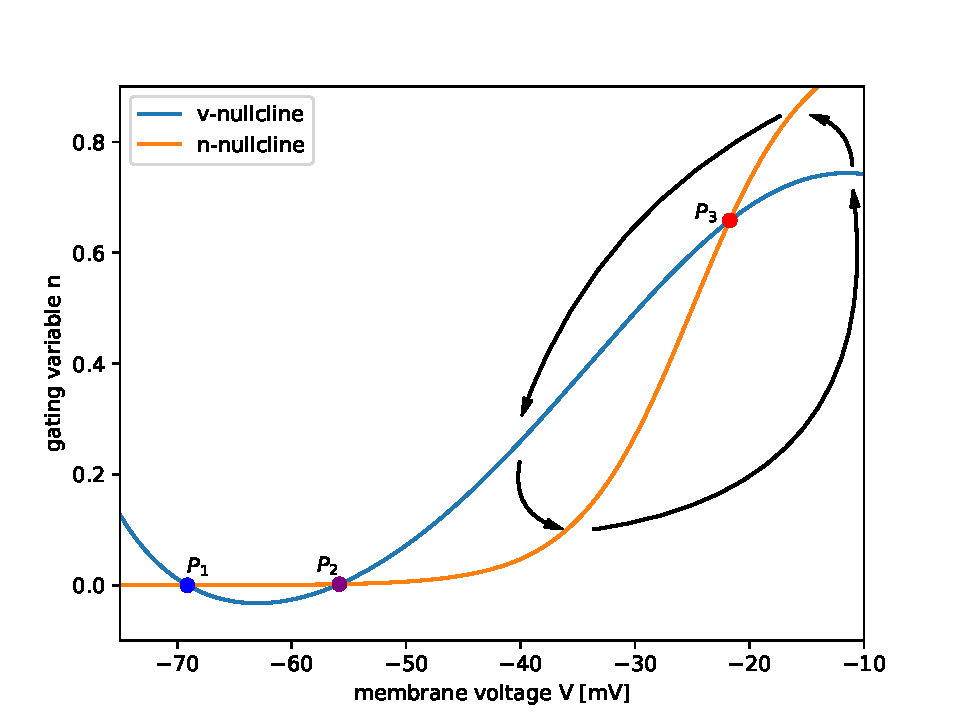
\includegraphics[scale=0.5]{Isoklinen.pdf}\caption{Isoklinen des $I_{Na,p}+I_K$-Modells bei $I=0$. Die Pfeile geben die Bewegungsrichtung in den verschiedenen Bereichen an und beschreiben eine mögliche burstende Trajektorie.}
	\label{realnc}
\end{figure}
Aus den Schnittpunkten der Isoklinen ergeben sich 3 Gleichgewichtspunkte: $P_1$ ist ein stabiler Knoten, $P_2$ ist ein Sattelpunkt und $P_3$ ist ein instabiler Fokus. 
\subsection{Phänomenologie des deterministischen Systems}
Abhängig von der Wahl der Startparameter geht das rauschlose System entweder in den ruhenden oder den laufenden Zustand über und verweilt in diesem. Misst man für verschiedene Kombinationen von Startparametern die Anzahl der Spikes über einen kurzen Zeitraum, erhält man eine Unterteilung des Phasenraums in die zwei entsprechenden Domänen.
\begin{figure}[H]
	\hspace*{-0.5cm}
	\subfigure[]{	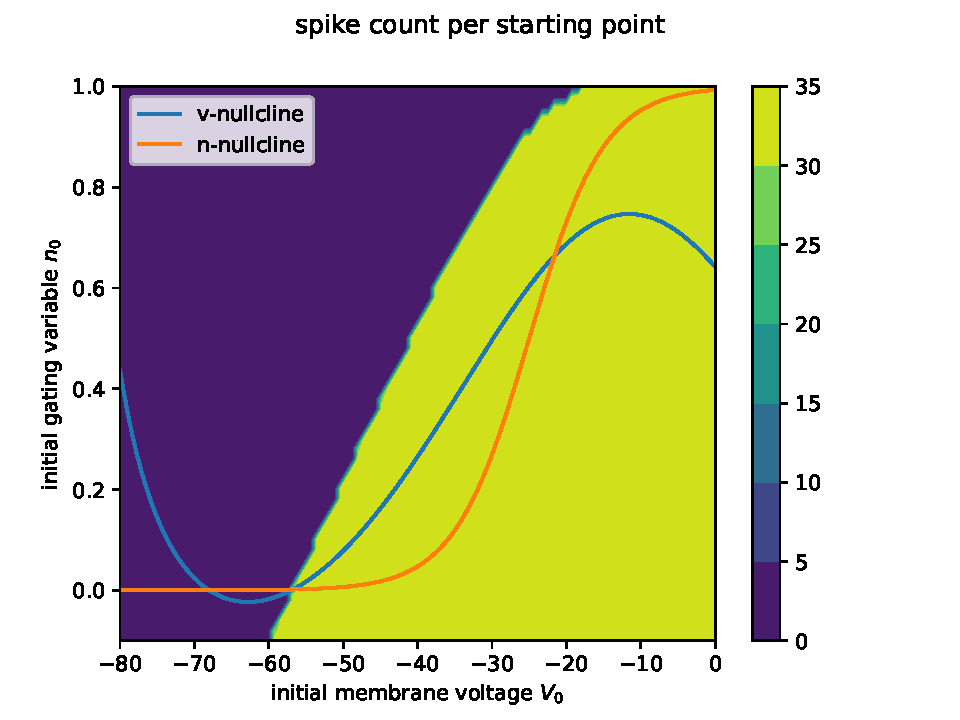
\includegraphics[scale=0.5]{Startparam_lang.pdf}}
	\subfigure[]{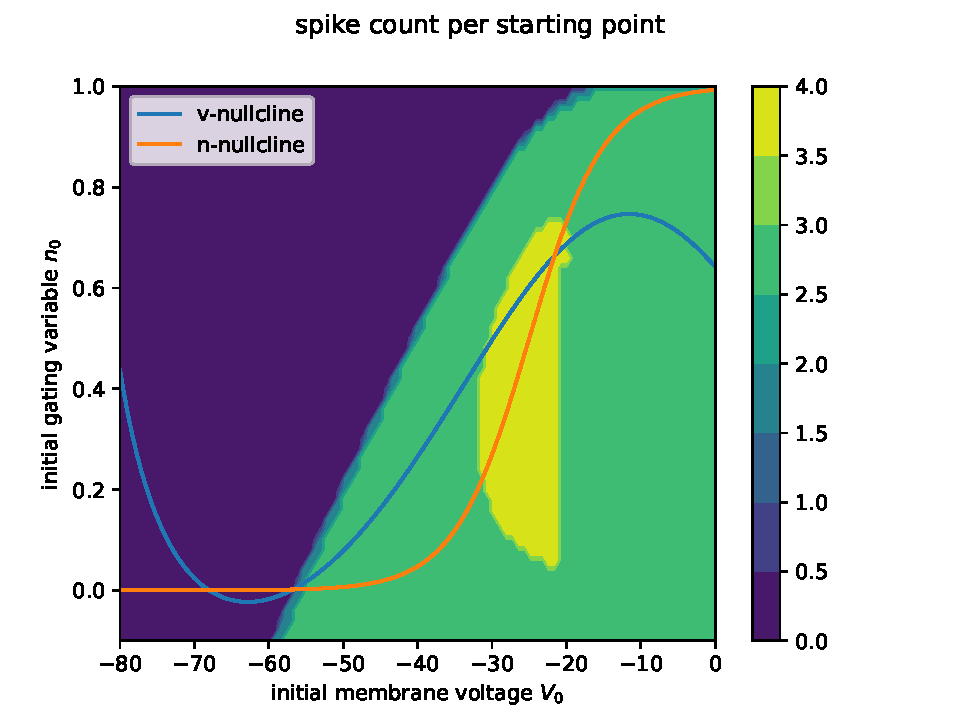
\includegraphics[scale=0.5]{Startparam_kurz.pdf}}
	
	\caption{Phasenraumbild des Nervenmodells mit $I=0.1$ und ohne Rauschen. Jeder Punkt stellt die Anzahl der Spikes über einen kurzen Zeitraum für eine bestimmte Kombination von Startparametern dar. Im linken Bild wurde eine Simulationszeit von 500 ms gewählt, im rechten nur 50 ms. Unregelmä"sigkeiten entstehen durch die endliche Auflösung des $V_0$-$n_0$-Rasters.}
	\label{twodom}
\end{figure}		
Die senkrechte Grenze im rechten Bild ist auf das Kriterium für die Registrierung eines Spikes zurückzuführen: Eine bestimmte Trajektorie wurde dann als Spike gewertet, wenn zunächst der Spannungswert des instabilen Fokus passiert wurde und anschlie"send der entsprechende Wert der Gatingvariable.
\subsection{Verhalten unter Rauschen}
Fügt man dem System Rauschen hinzu, ist eine eindeutige Zuordnung zwischen Startparametern und finalem Zustand nicht mehr möglich, es finden ständig rauschinduzierte Wechsel zwischen beiden Zuständen statt.
\begin{figure}[H]
	\hspace*{-0.5cm}
	\subfigure[]{	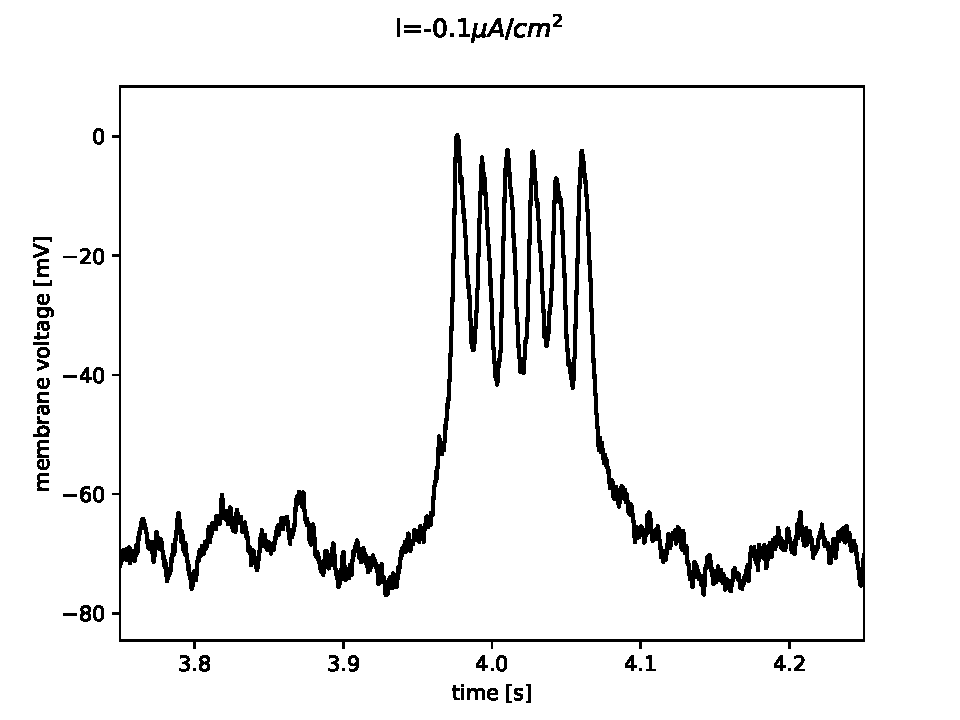
\includegraphics[scale=0.5]{V-t-diagramm.pdf}}
	\subfigure[]{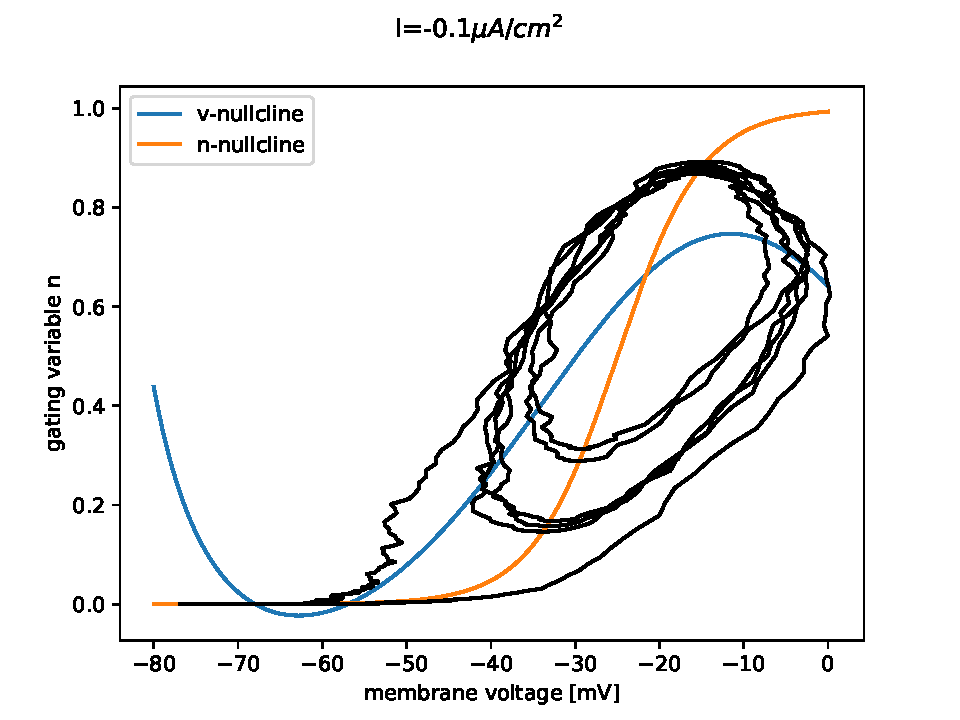
\includegraphics[scale=0.5]{n-V-diagramm.pdf}}
	\caption{Vergleich zwischen zeitlichem Verlauf der Membranspannung und der zeitgleichen Trajektorie im Phasenraum bei gro"ser Rauschintensit"at ($D=1$). Der Zustandsvektor beschreibt zunächst 4 weite Kurven, wird dann auf eine engere Bahn gebracht und geht nach zwei weiteren Umläufen in den Ruhezustand über.}
	\label{trans}
\end{figure}
In der Regel wird dabei einer der beiden Zustände bevorzugt. Zu erwarten ist, dass bei geringem Bias-Strom $I$ der Ruhezustand dominiert und bei hohem $I$ der laufende Zustand. Wählt man einen etwas grö"seren Ma"sstab, kann man eine Tendenz über mehrere Wechsel erkennen.
\begin{figure}[H]
	\subfigure[]{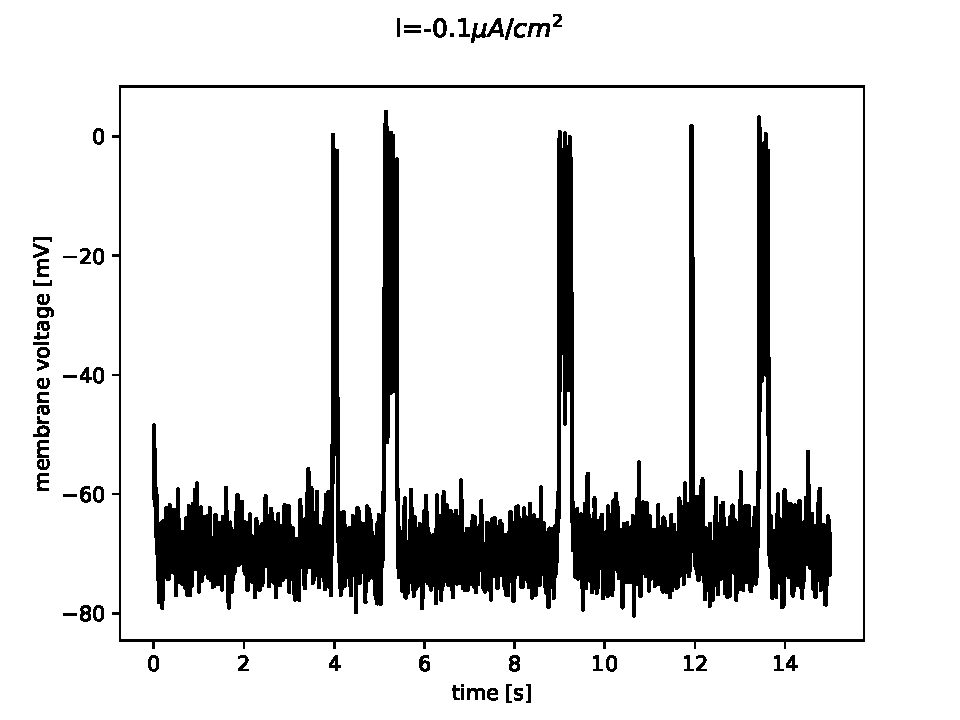
\includegraphics[scale=0.4]{uebergaengeI=-0,1.pdf}} 
	\subfigure[]{	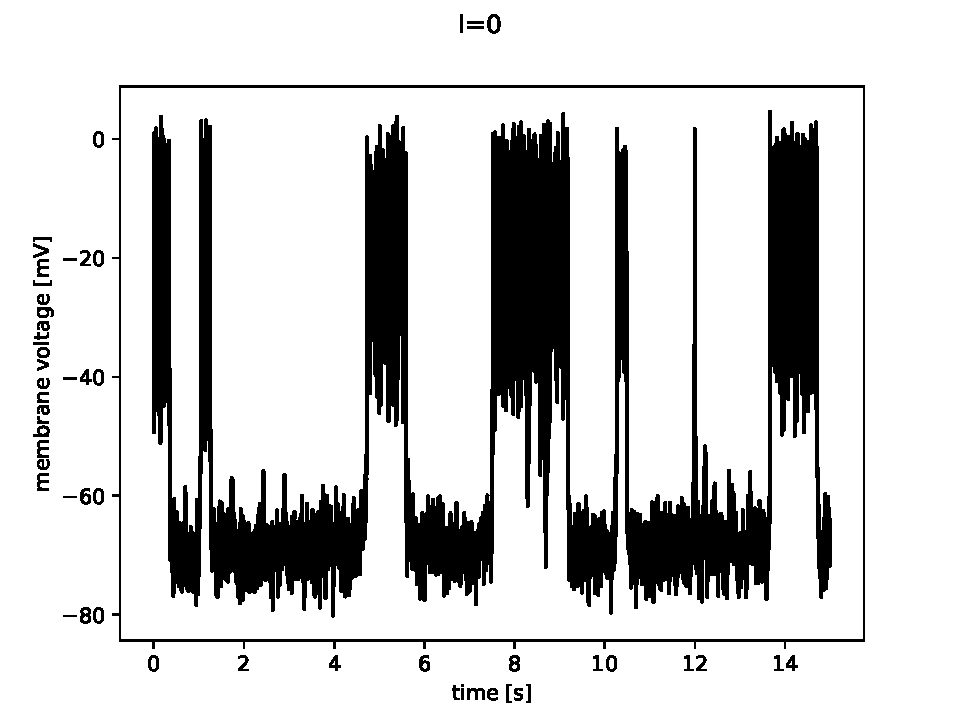
\includegraphics[scale=0.4]{uebergaengeI=0.pdf}}\\	\subfigure[]{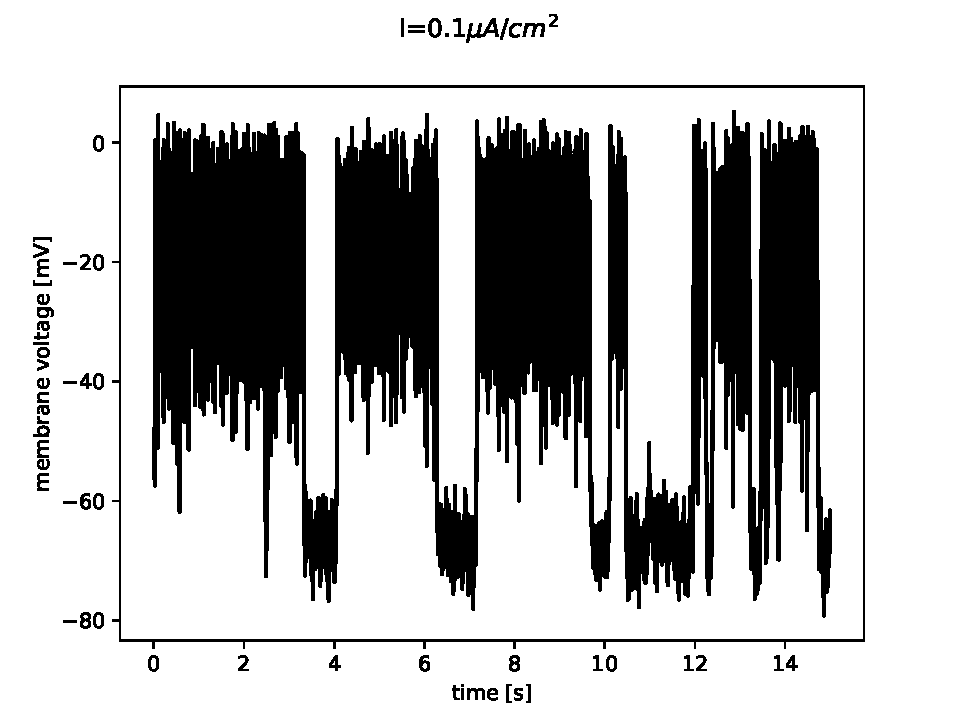
\includegraphics[scale=0.4]{uebergaengeI=0,1.pdf}} 
	\subfigure[]{	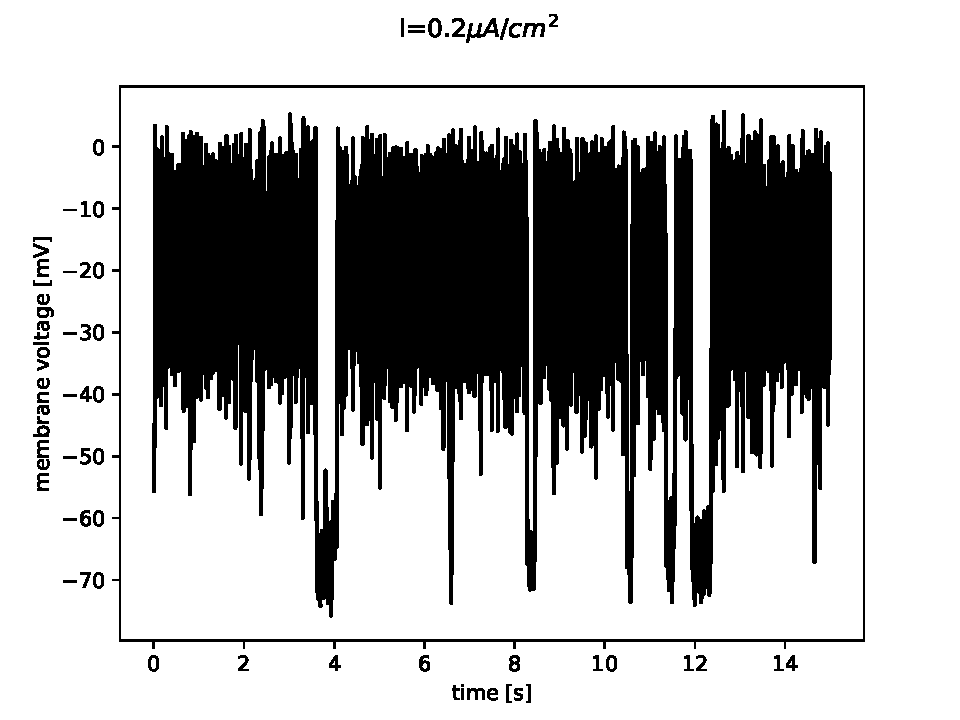
\includegraphics[scale=0.4]{uebergaengeI=0,2.pdf}}
	\caption{Verhalten der Membranspannung bei $D=1$ und wechselndem Bias-Strom $I$. Die Rauschintensität wurde so hoch gewählt, damit über einen geringen Zeitraum viele Wechsel zu beobachten sind.}
	\label{currentnoise} 
\end{figure}
Die anfänglichen Vermutungen werden somit bestätigt: bei geringem Strom verweilt das System kaum in dem laufenden Zustand, und bei hohem Strom verweilt es fast ausschließlich in diesem.
\section{Zählstatistik}
Simuliert man das Neuronenmodell über einen Bereich von Bias-Strömen und berechnet Diffusionskoeffizient, Feuerrate und Fano-Faktor, so erhält man folgende Resultate:
\begin{figure}[H]
	\centering
	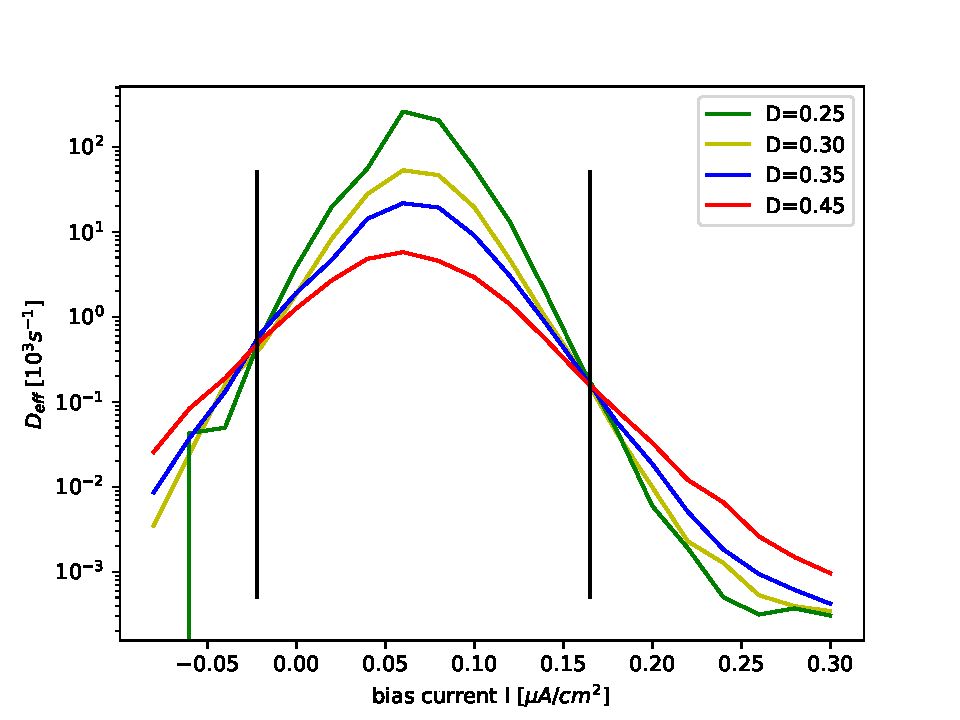
\includegraphics[scale=0.5]{deff.pdf}\caption{Diffusionskoeffizienten für verschiedene Rauschintensitäten}
	\label{deff}
\end{figure}
Hier sind zwei Bereiche des gerichteten Transports und ein Gebiet mit Giant Diffusion sichtbar.
\begin{figure}[H]
	\centering
	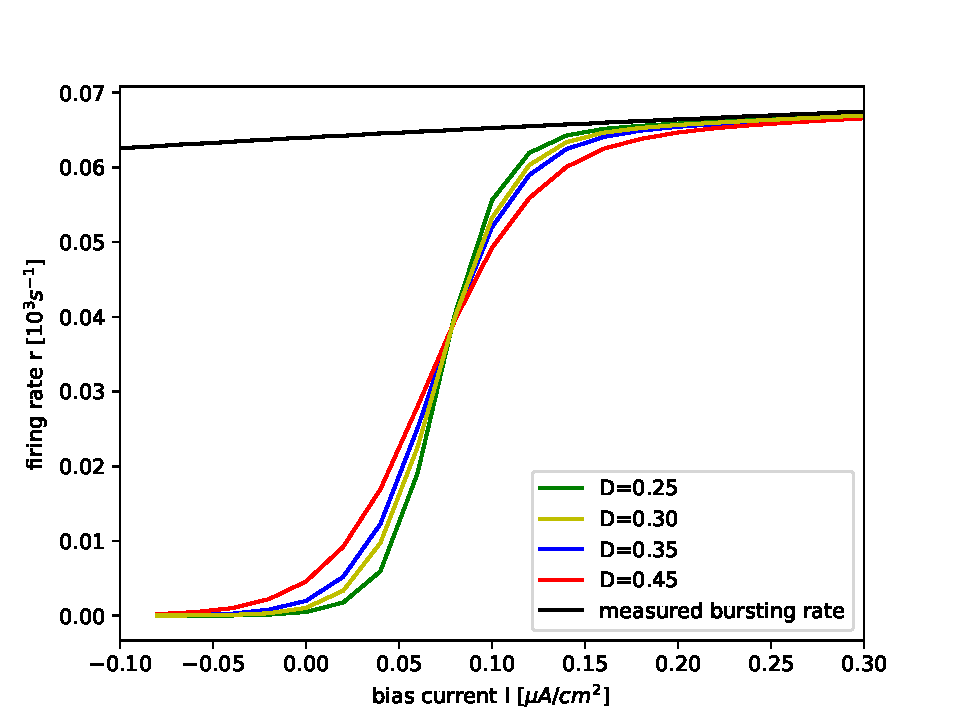
\includegraphics[scale=0.5]{firingrate.pdf}\caption{Mittlere Feuerraten für verschiedene Rauschintensitäten}
	\label{firate}
\end{figure}
Alle Feuerraten schneiden sich in einem gemeinsamen Punkt und konvergieren mit zunehmendem $I$ gegen die Feuerrate im laufenden Zustand.
\begin{figure}[H]
	\centering
	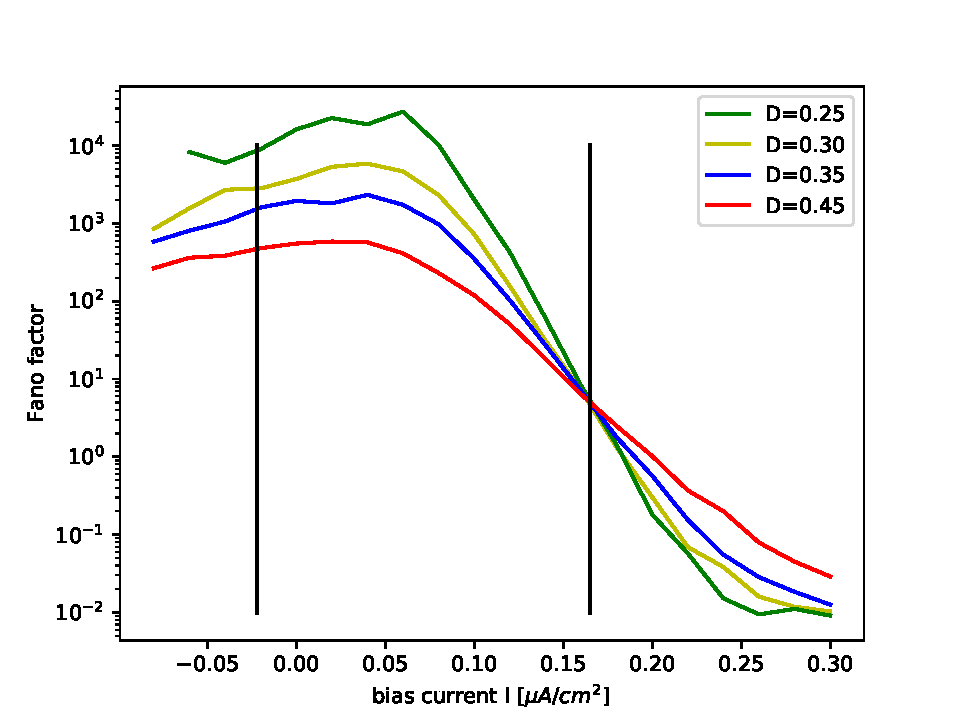
\includegraphics[scale=0.5]{fano.pdf}\caption{Fano-Faktoren für verschiedene Rauschintensitäten}
	\label{fano}
\end{figure}
Während bei geringem Strom kein Schnittpunkt der Kurven mehr existiert, fällt der Schnitpunkt bei hohem Strom mit dem Schnittpunkt der Diffusionskoeffizienten zusammen.
Durch die geringe Anzahl an Wechseln zwischen den Zuständen ist die Kurve für $D=0.25$ im Randbereich leicht verrauscht.
\\
\subsection{Übergangsraten}
Neben der Anzahl an Spikes kann man noch andere Grö"sen messen, zum Beispiel die Übergangsraten zwischen den beiden Zuständen. Das System befindet sich im ruhenden Zustand, wenn es in beliebiger Reihenfolge $n$- und $V$- Wert des stabilen Knotens überquert hat. Im laufenden Zustand ist es, wenn es gerade einen Spike erzeugt hat, also zunächst den $V$- Wert des instabilen Fokus und danach dessen $n$- Wert passiert hat. Indem man die Zeitpunkte dieser Wechsel festhält, kann man dann die Übergangsraten bestimmen. Demnach gibt es für jeden Wert des Bias-Stromes $I$ Übergangsraten für mehrere Werte von $D$. Für diese biete sich die Darstellung in einem Arrhenius-Plot an.
\subsubsection{Interburst-Intervalle}
\begin{figure}[H]
	\centering
	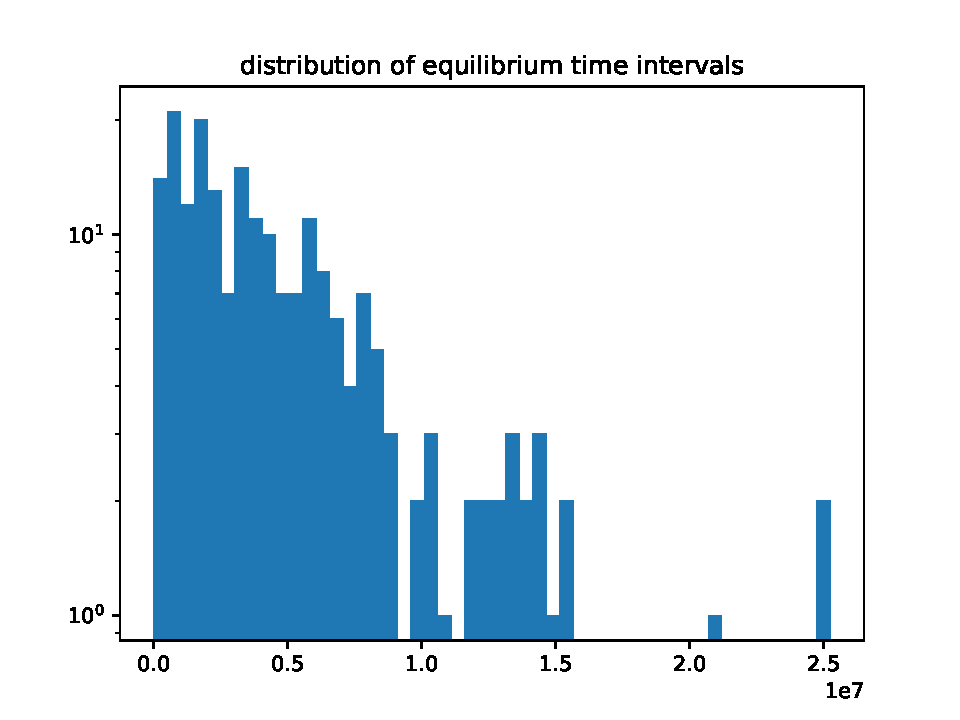
\includegraphics[scale=0.5]{eqdistajrj2newrealfast11jjem2sh352.pdf}\caption{Verteilung der Interburst-Intervalle bei $D=0.35$ und $I=-0.06$}
	\label{hist35bad}
\end{figure}
\begin{figure}[H]
	\centering
	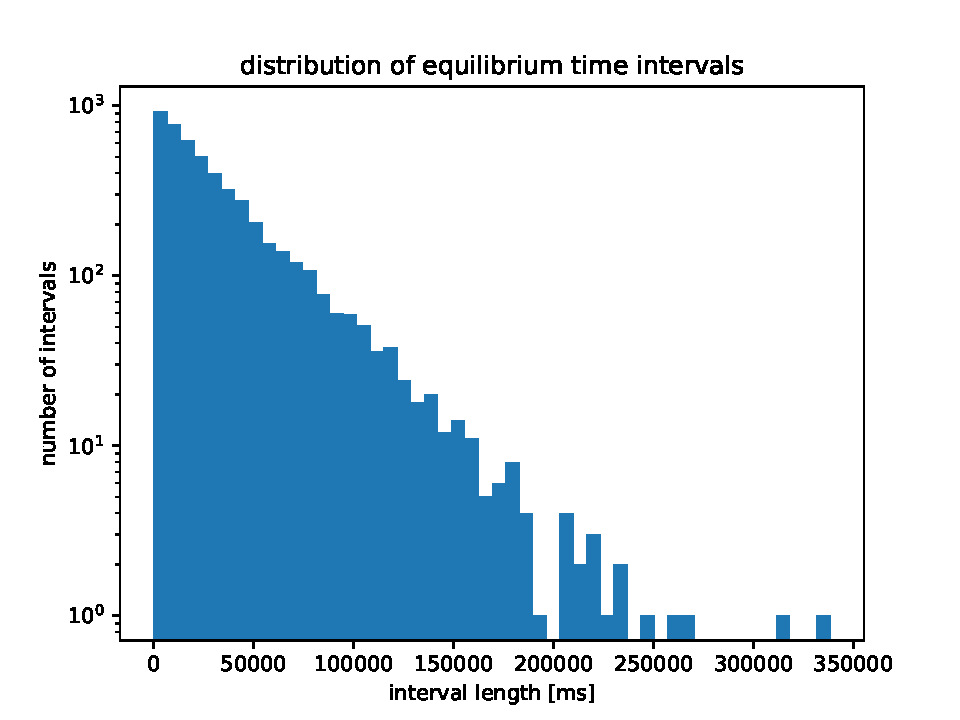
\includegraphics[scale=0.5]{eqdistajrj2newrealfast11jjem2sh359.pdf}\caption{Verteilung der Interburst-Intervalle bei $D=0.35$ und $I=0.08$}
	\label{hist35}
\end{figure}
\begin{figure}[H]
	\centering
	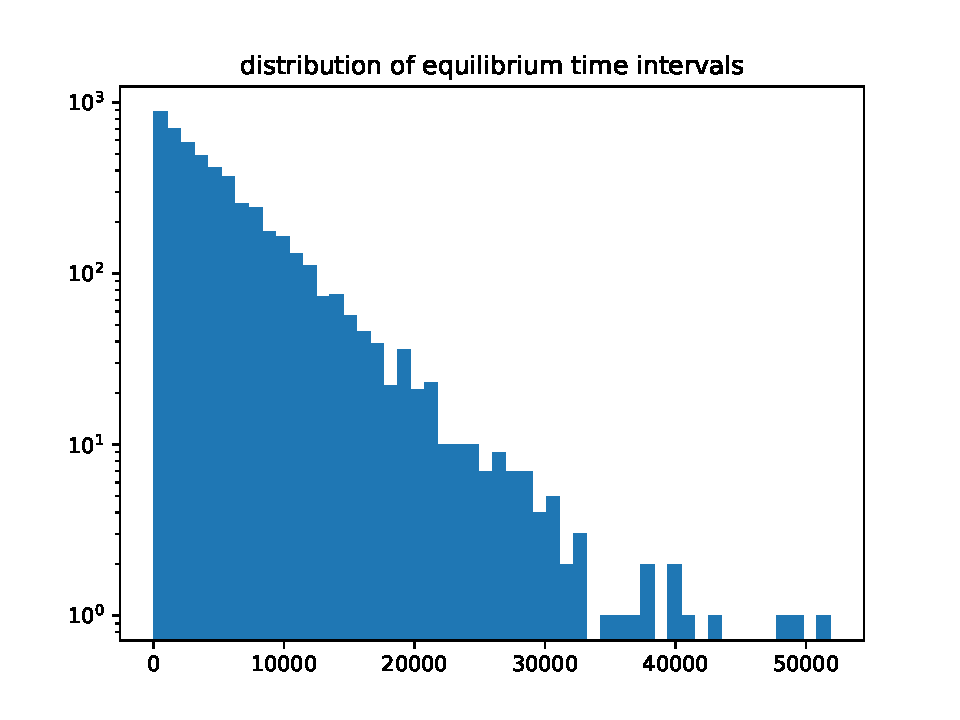
\includegraphics[scale=0.5]{eqdistajrj2newrealfast11jjem2st509.pdf}\caption{Verteilung der Interburst-Intervalle bei $D=0.5$ und $I=0.08$}
	\label{hist50}
\end{figure}
\subsubsection{Extraktion der Potentialbarrieren}
F"ur die "Ubergangsraten wird eine Arrhenius-Gleichung angenommen:
\begin{align*}
w_{\pm}=w_{0,\pm}\text{e}^{-\frac{\Delta U_{\pm}}{D}}
\end{align*}
An jedem Wert für $I$ wird ein Satz aus den Raten aller verschiedenen Diffusionskoeffizienten mit dieser Gleichung gefittet. Neben den Vorfaktoren der Raten kann man so auch Werte für effektive Potentialbarrieren bestimmen.
\begin{figure}[H]
	\subfigure[]{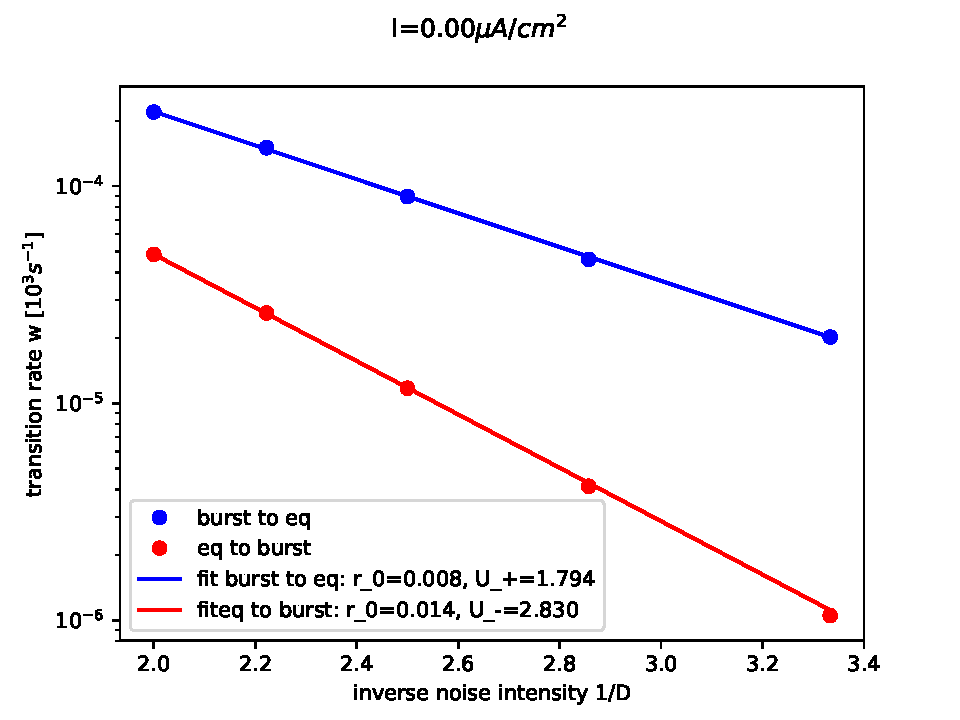
\includegraphics[scale=0.4]{ArrheniusI=0.pdf}} 
	\subfigure[]{	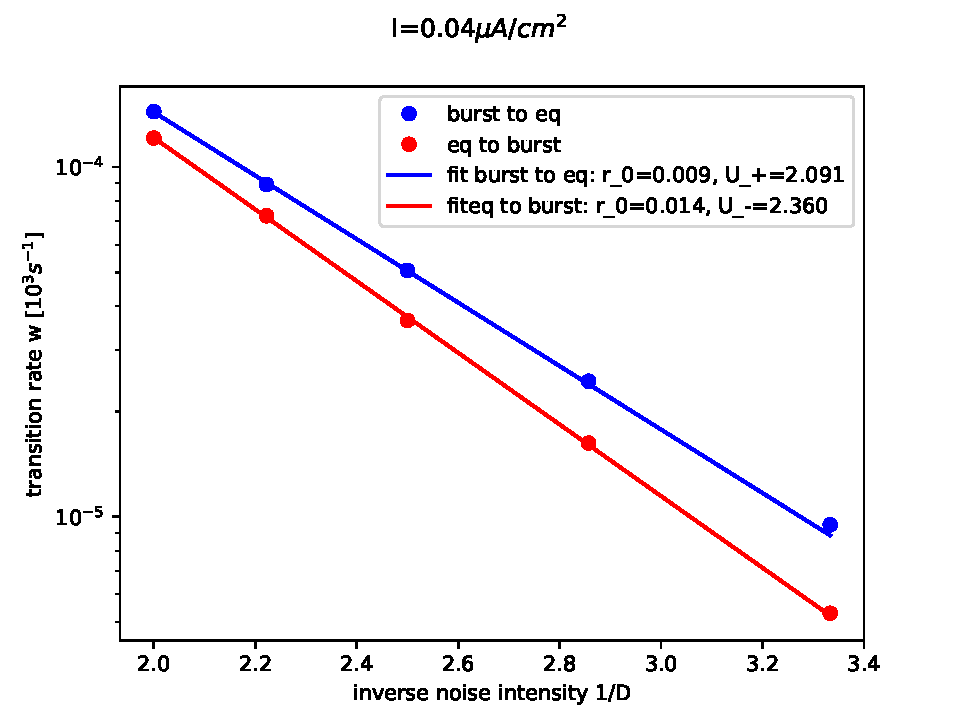
\includegraphics[scale=0.4]{ArrheniusI=0,04.pdf}}\\	\subfigure[]{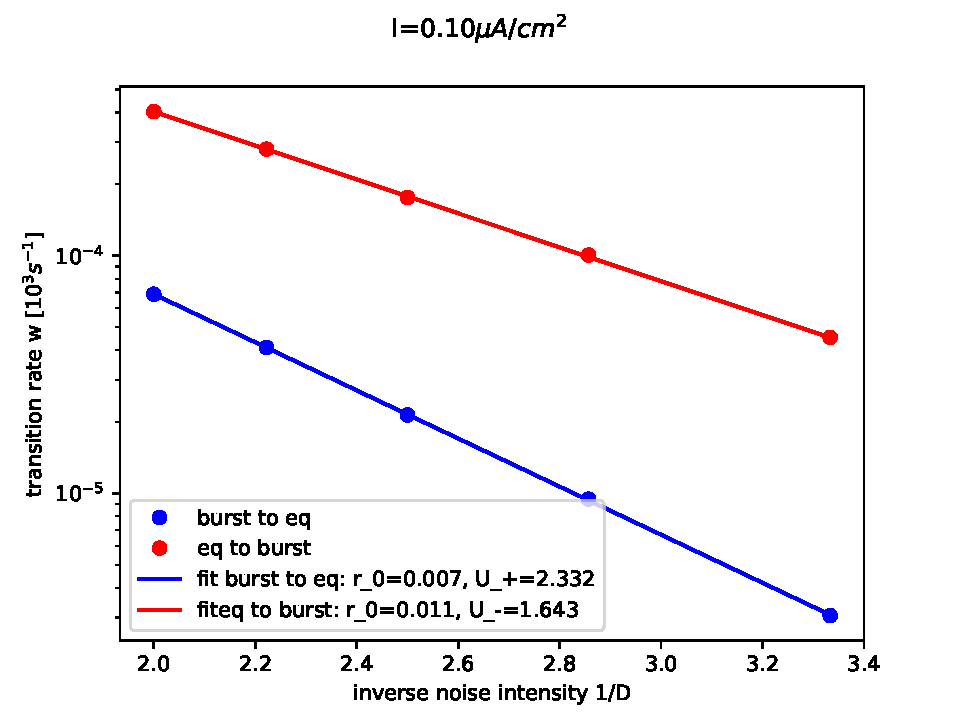
\includegraphics[scale=0.4]{ArrheniusI=0,1.pdf}} 
	\subfigure[]{	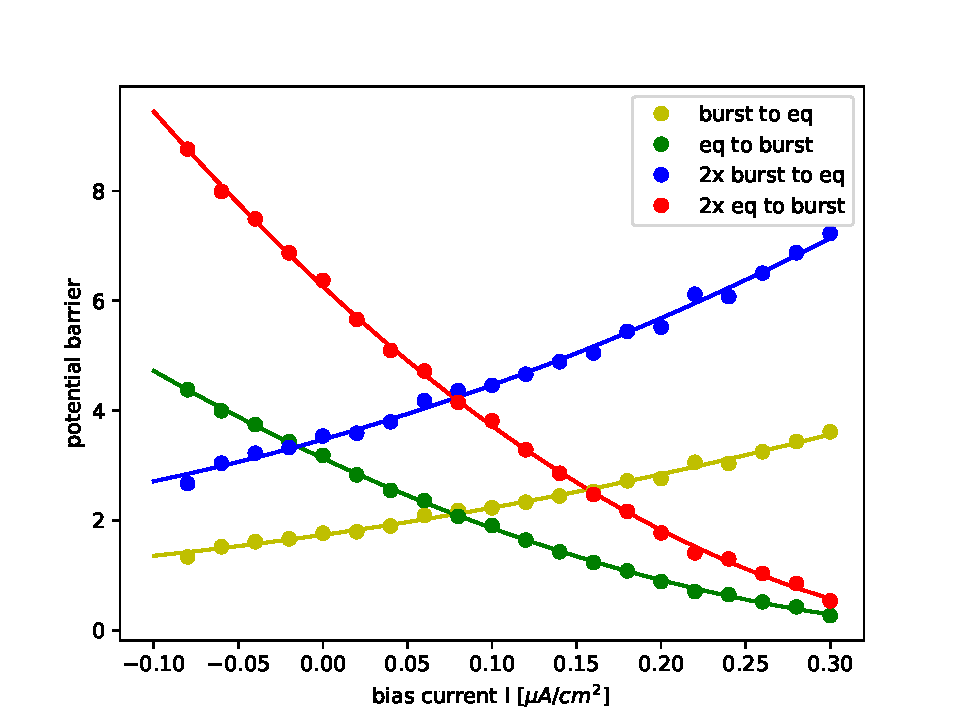
\includegraphics[scale=0.4]{potbarriersfit.pdf}}
	\caption{Arrhenius-Plots mit beiden Übergangsraten und den Kramers-Fits. Bild (d) zeigt die daraus extrahierten Barrieren, die mit einfachen quadratischen Funktionen gefittet wurden}
	\label{arrhstuff} 
\end{figure}
Offensichtlich steigen die Übergangsraten mit der Rauschintensität. Zudem ist bei geringem $I$ die Übergangsrate zum ruhenden Zustand höher als die andere, bei moderatem Bias-Strom sind beide Raten in etwa gleich gro"s, und bei noch höherem Strom ist die Übergnagsrate zum burstenden Zustand am Grö"sten. Diese Beobachtungen passen auch zu den extrahierten Potenitalbarrieren: während die Potentialbarriere zum Gleichgewichstzustand mit dem Strom ansteigt, nimmt die Potentialbarriere zum laufenden Zustand ab. \\
Mit der Kenntnis dieser Raten lässt sich nun die Gültigkeit der Zwei-Zustands-Theorie überprüfen. In dieser wird der Diffusionskoeffizient durch die Übergansraten wir folgt beschrieben:
\begin{align*}
D_{\text{eff}}=\frac{(r_+-r_-)^2 w_+w_-}{(w_++w_-)^3}=\frac{r_+^2 w_+w_-}{(w_++w_-)^3}
\end{align*}
wobei $r_\pm$ die Feuerraten im laufenden bzw ruhenden Zustand bezeichnet. Unter der Annahme, dass im ruhenden Zustand keine Spikes gefeuert werden, lässt sich dieser Beitrag vernachlässigen. Die mittlere Feuerrate ergibt sich demnach lediglich noch aus der Zeit, die das System im laufenden Zustand verbringt:
\begin{align*}
r=r_+\frac{w_-}{w_++w_-}
\end{align*}
und der Fano-Faktor ergibt sich aus dem Quotienten von $D_{eff}$ und $r$:
\begin{align*}
F=\frac{2D_{eff}}{r}
\end{align*}
Vergleicht man nun die Messergebnisse Punkt für Punkt (also $I$-Wert für $I$-Wert) mit der Zwei-Zustands-Theorie, ergeben sich folgende Bilder:
\begin{figure}[H]
	\centering
	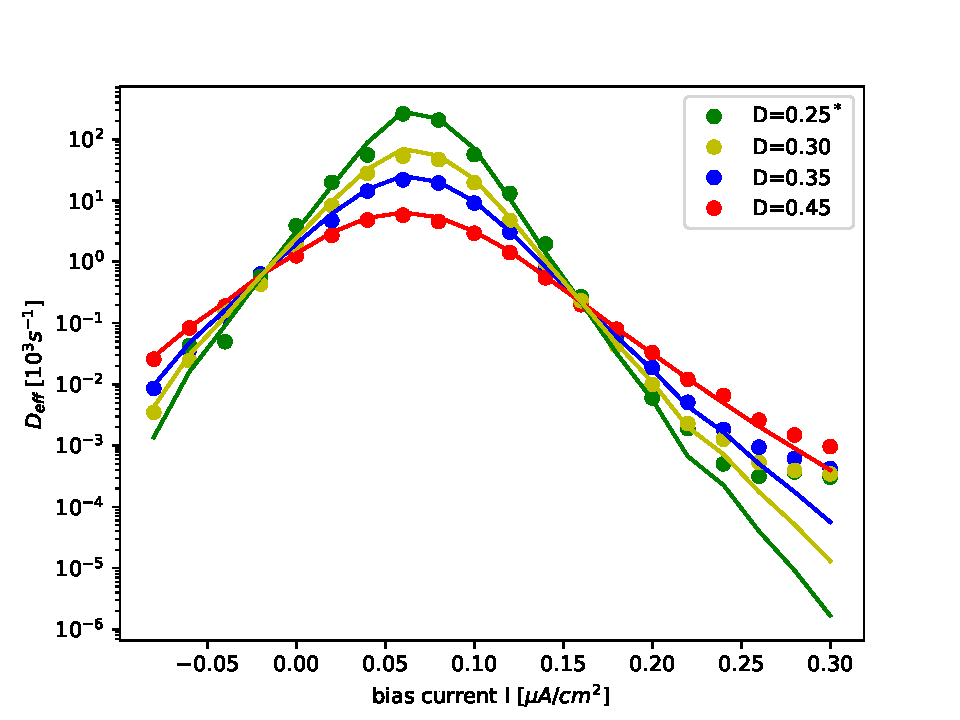
\includegraphics[scale=0.5]{deffnofit.pdf}\caption{Vergleich der Diffusionskoeffizienten mit der Zwei-Zustands-Theorie. Die Werte für $D=0.25$ wurden aus den Raten der anderen Rauschintensitäten vorhergesagt.}
	\label{dcomp}
\end{figure}
\begin{figure}[H]
\centering
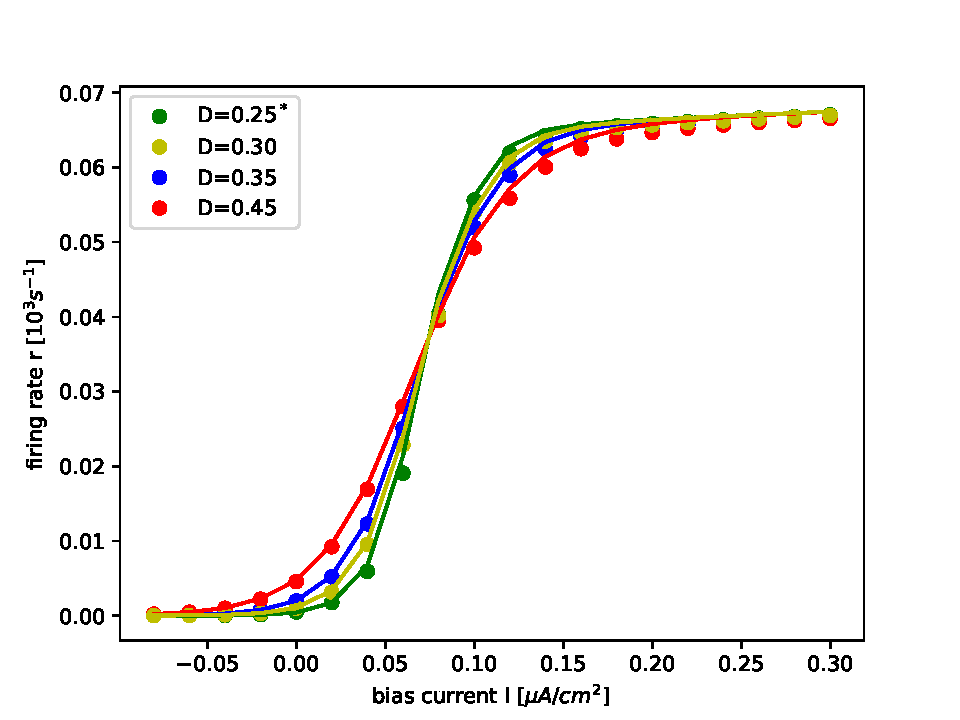
\includegraphics[scale=0.5]{ratenofit.pdf}\caption{Vergleich der Feuerraten mit der Zwei-Zustands-Theorie}
\label{gcomp}
\end{figure}
\begin{figure}[H]
	\centering
	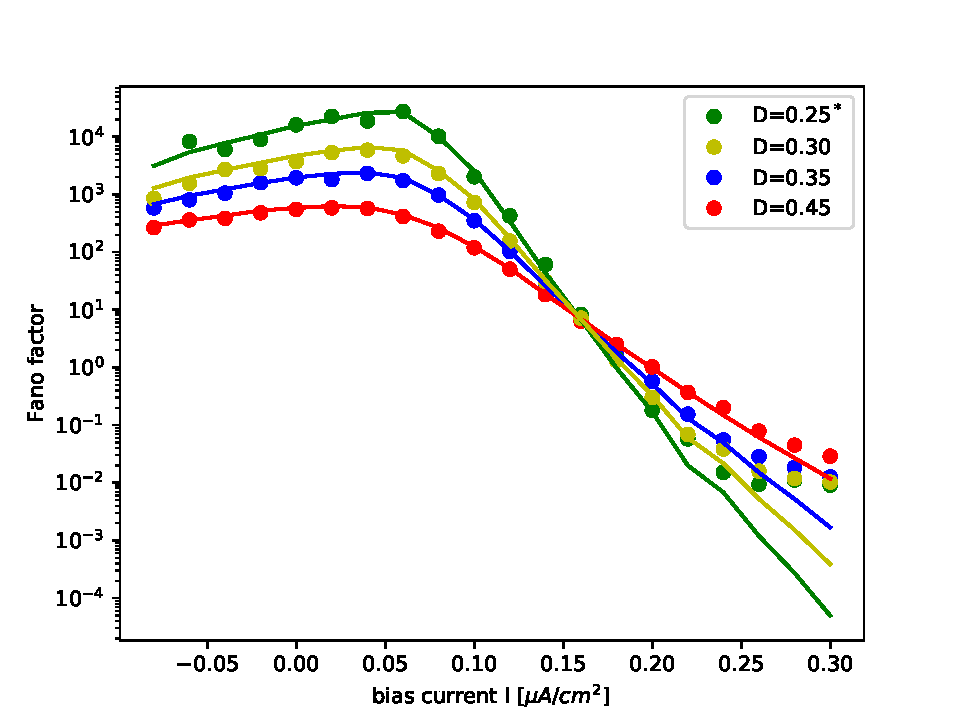
\includegraphics[scale=0.5]{fanonofit.pdf}\caption{Vergleich Fano-Faktor mit Zwei-Zustands-Theorie}
	\label{fanocomp}
\end{figure}
Bis auf einige Punkte bei $I>0.2$ scheint die Zwei-Zustands-Theorie eine gute Beschreibung des vorliegenden Systems zu liefern. Damit kann diese Theorie nun genutzt werden, um Vorhersagen für das Verhalten bei noch geringeren Rauschintensitäten zu treffen:
\begin{figure}[H]
	\centering
	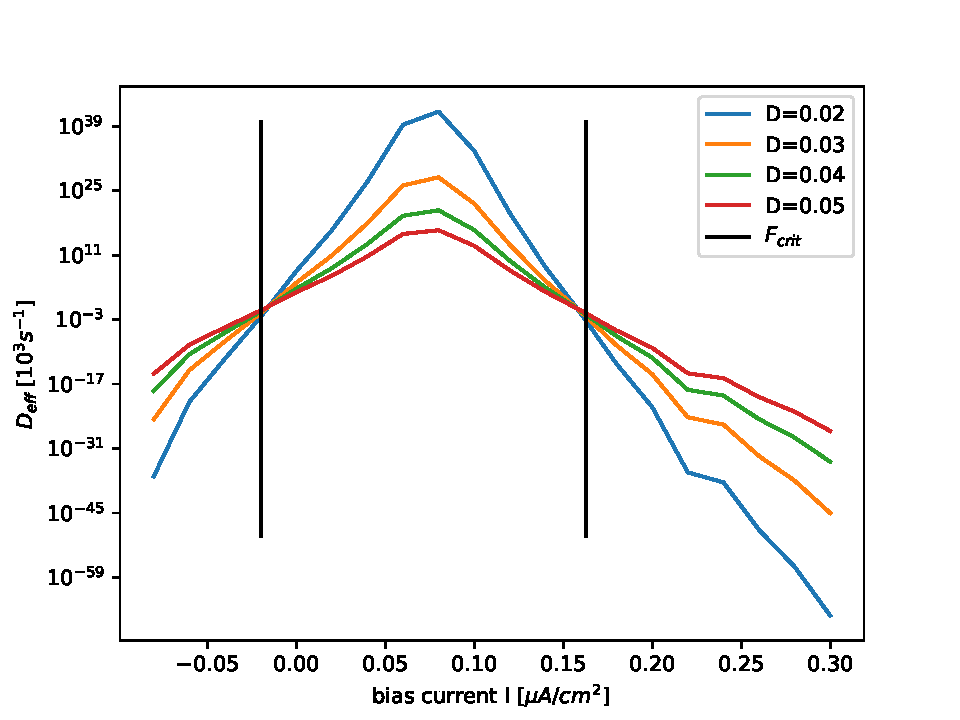
\includegraphics[scale=1]{deffpred.pdf}\caption{Vorhersage des Diffusionskoeffizienten für geringe Rauschintensitäten}
	\label{deffpred}
\end{figure}
Es zeigt sich, dass die gemeinsamen Schnittpunkte sich noch etwas weiter zur Mitte verschieben, sonst ändert sich allerdings nichts.
\subsection{Spektrum und SNR}
Die gewonnenen Erkenntnisse legen nahe, dass innerhalb des Bereichs der Giant Diffusion nur eine schlechte Signalübertragung möglich ist, während das SNR au"serhalb davon exponentiell ansteigen müsste. Um dies zu überprüfen, wird das Feuern des Neurons durch einen Spike-Train angenähert und das Power-Spektrum davon ermittelt.
\begin{figure}[H]
	\hspace*{-0.5cm}
	\subfigure[]{	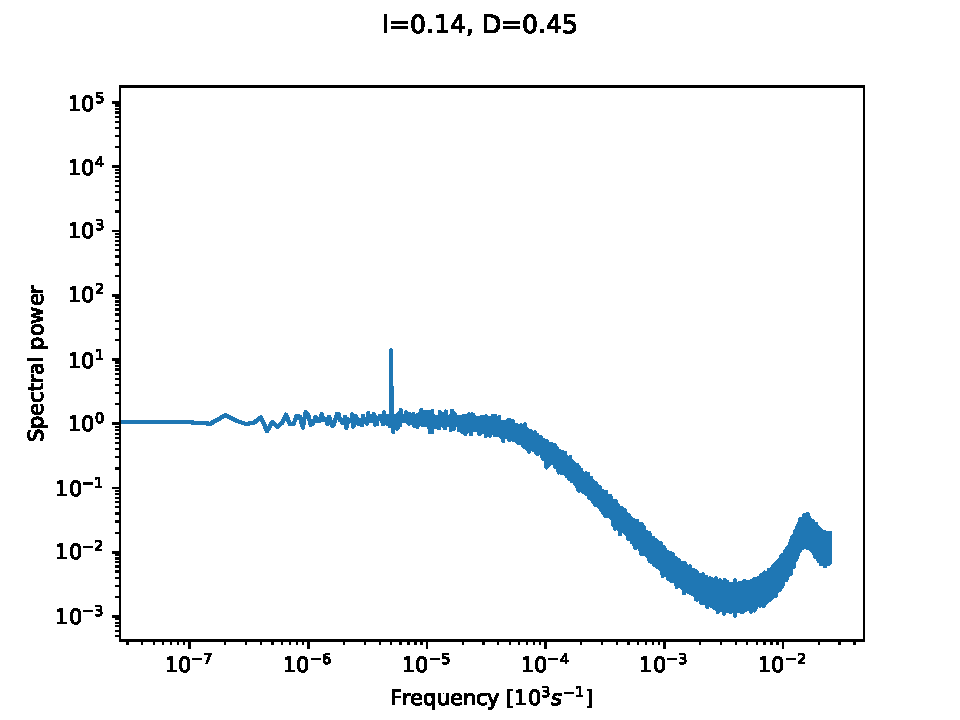
\includegraphics[scale=0.5]{spektrumD=0,45I=0,14.pdf}}
	\subfigure[]{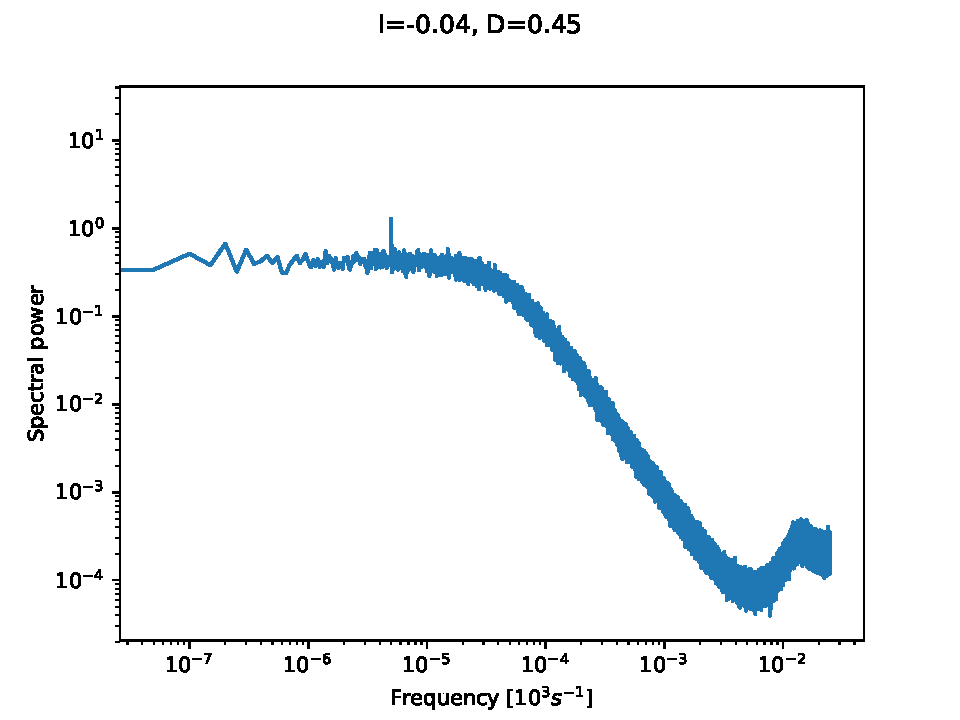
\includegraphics[scale=0.5]{spektrumD=0,45I=-0,04.pdf}}
	\caption{}
	\label{spec}
\end{figure}
Obwohl in beiden Fällen mit einem periodischen Signal der Frequenz $\Omega=5*10^{-6}$ angeregt wurde, ist der Delta-Peak bei geringem Strom stärker ausgeprägt. Bei verschieden Werten von $D$ hat das SNR dieselben qualitativen Eigenschaften:
\begin{figure}[H]
	\centering
	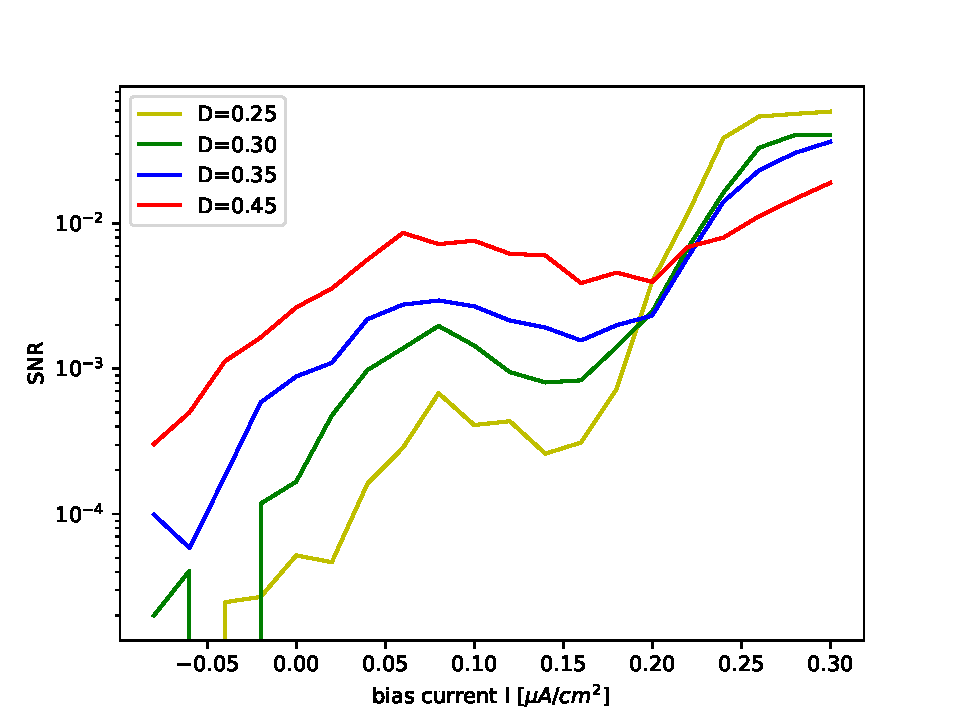
\includegraphics[scale=1]{snronly.pdf}\caption{SNR für verschiedene Rauschintensitäten bei konstantem Signal der Stärke $\epsilon=0.01 \mu A/cm^2$}
	\label{snr}
\end{figure}
Es gibt ein ausgeprägtes Maximum und zwei Minima, und in den Randbereichen steigt das SNR an. 
\\
Das Signal-zu-Rausch Verhältnis kann für ein Kosinus-Signal mit Stärke $\epsilon$ folgenderma"sen berechnet werden:
\begin{align*}
SNR=\frac{\epsilon ^2T}{4}\frac{|\chi(\omega)|^2}{S_0(\omega)}=\frac{\epsilon^2T|dr/dI|^2}{8\cdot D_{eff}}
\end{align*}
Wenn man die Ableitung der Feuerrate numerisch aus vorherigen Messungen bestimmt und den gemessenen Diffusionskoeffizienten verwendet, lässt sich eine gute Vorhersage des SNR treffen:
\begin{figure}[H]
	\centering
	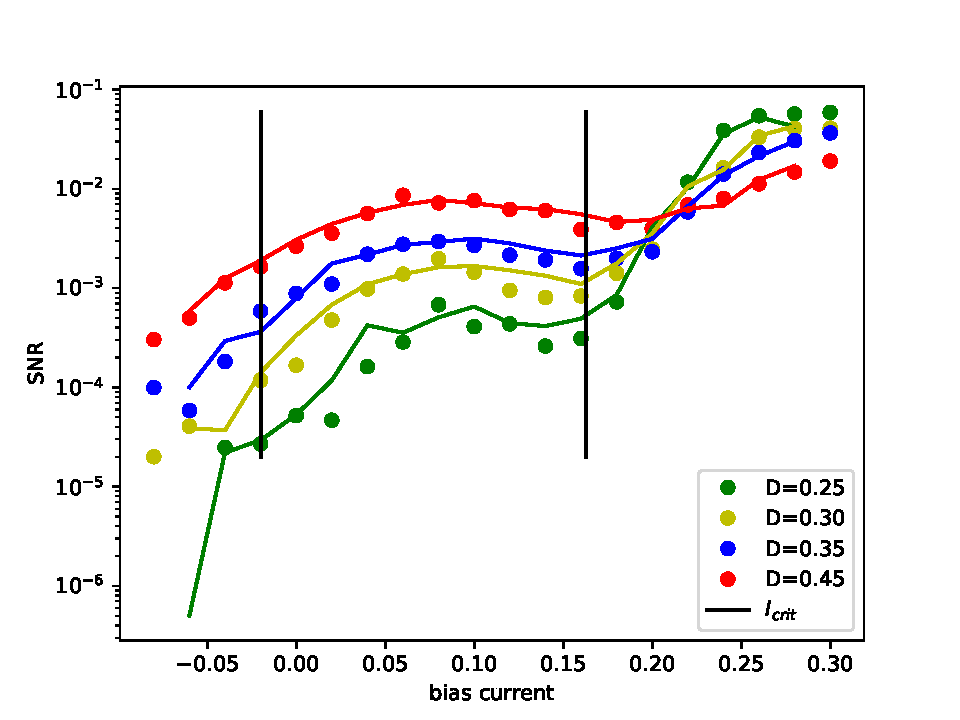
\includegraphics[scale=1]{snrdeffrate.pdf}\caption{Vergleich des SNR mit dem Schätzwert aus $D_{eff}$ und der numerisch bestimmten Ableitung von $r$}
	\label{snrdeffrate}
\end{figure}
Eine zweite Variante ist erneut die Zwei-Zustands-Theorie. Dafür wird lediglich noch die Ableitung der mittleren Feuerrate benötigt:
\begin{align*}
\frac{dr}{dI}&=\frac{d}{dI}\left(\frac{r_+w_-}{w_++w_-}\right)=\frac{r_+'w_-}{w_++w_-}+\frac{r_+w_-'}{w_++w_-}-\frac{r_+w_-(w_+'+w_-')}{(w_++w_-)^2}\\
&=\frac{r_+'w_-}{w_++w_-}+\frac{r_+(w_+w_-'-w_-w_+')}{(w_++w_-)^2}
\end{align*}
Die Ableitung von $r_+$ ist bereits (numerisch) bekannt, und die Ableitungen der Raten sind durch
\begin{align*}
w_\pm'=\frac{w_{0,\pm}'}{w_{0,\pm}}w_\pm-\frac{\Delta U_\pm'}{D}w_\pm=\left(\frac{w_{0,\pm}'}{w_{0,\pm}}-\frac{\Delta U_\pm'}{D}\right)w_\pm
\end{align*}
gegeben. Die Ableitungen von Vorfaktor und Potential können erneut numerisch für jeden Wert von $I$ bestimmt werden. Die Zwei-Zustands-Theorie liefert wieder bis ca $I=0.2$ eine sehr gute Übereinstimmung und der Verlauf der Kurve für $D=0.25$ kann gut vorhergesagt werden:
\begin{figure}[H]
	\centering
	\includegraphics[scale=1]{snrtwostate.pdf}\caption{Vergleich des SNR mit der Zwei-Zustands-Theorie}
	\label{snrtwostate}
\end{figure}
Auch hier bietet es sich daher an, den Verlauf für noch kleinere Werte von $D$ vorherzusagen:
\begin{figure}[H]
	\centering
	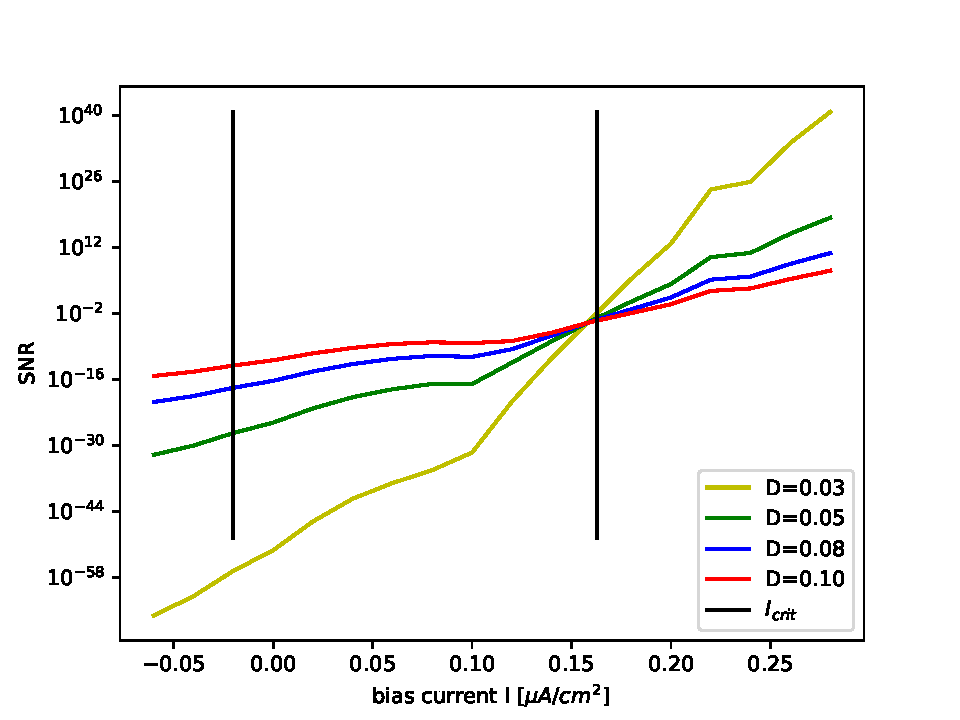
\includegraphics[scale=1]{SNRpred.pdf}\caption{SNR für niedrige Werte von $D$}
	\label{snrpred}
\end{figure}
Mit abnehmendem Rauschen wird das Verhalten des SNR immer monotoner: bei kleinen Strömen geht es gegen 0, und bei hohen Strömen steigt es exponentiell. Der Schnittpunkt aller Kurven verschiebt sich nach links und stimmt am Ende mit dem Schnittpunkt der Diffusionskoeffizienten überein.
\section{Andere bistabile Modelle}
Hodgkin-Huxley-Modell mit additivem Rauschen
\begin{figure}[H]
	\centering
	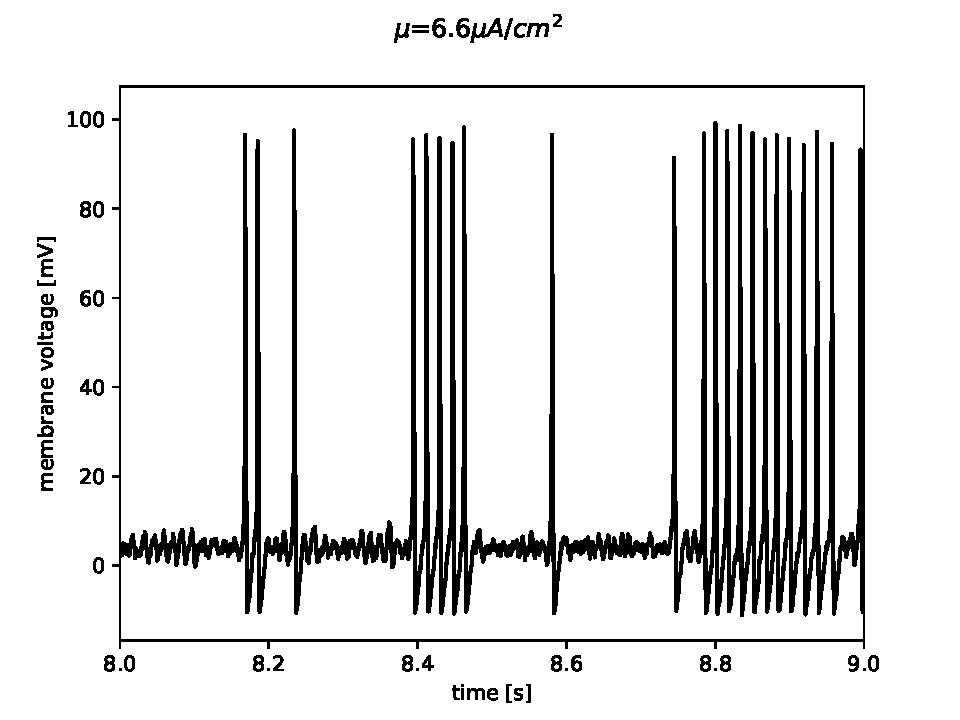
\includegraphics[scale=1]{realstatehhkurz.pdf}\caption{Verlauf der Spannungsvariablen im Hodgkin-Huxley Modell}
	\label{hhvolt}
\end{figure}
\begin{figure}[H]
	\centering
	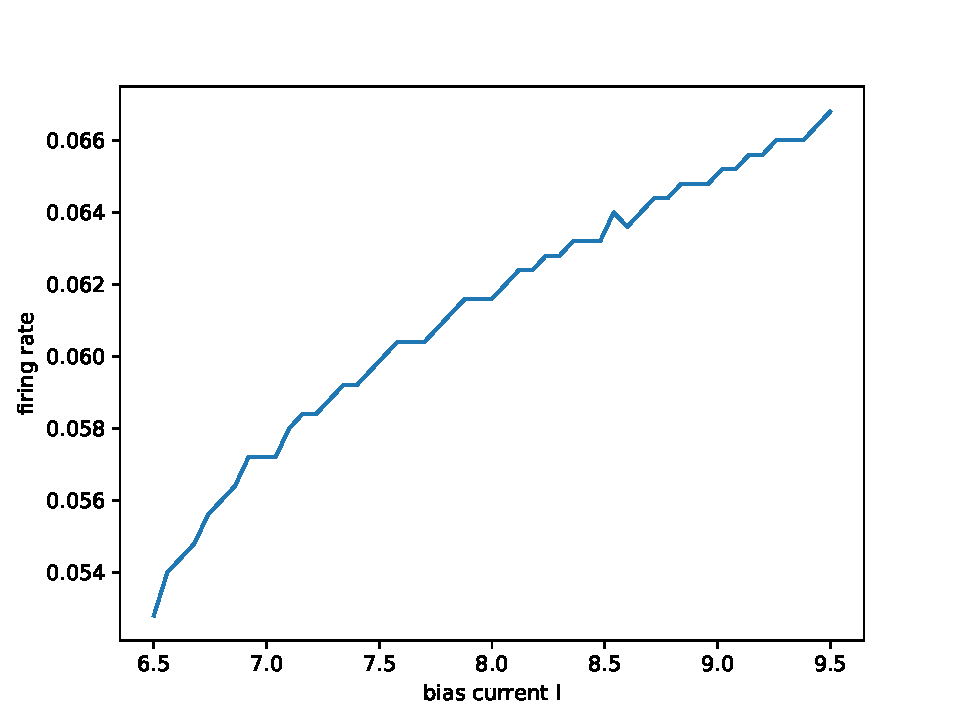
\includegraphics[scale=1]{detmocounthh.pdf}\caption{Verhalten der mittleren Feuerrate im H-H-Modell}
	\label{hhcount}
\end{figure}
FHN-artiges Modell des H-H-Modells nach Rinzel:
\begin{align*}
C\dot{V}&=I_{app}-g_{Na}m_\infty^3(V)(1-W)(V-V_Na)\\
&-g_K(W/S)^4(V-V_K)-g_L(V-V_L)\\
\dot{W}&=\phi\left[W_\infty(V)-W\right]/\tau(V)
\end{align*}
\begin{align*}
S=\frac{(1-h_\infty(0))}{n_\infty(0)}\\
W_\infty(V)=S\left(n_\infty(V)+S\left[1-h_\infty(V)\right]\right)/(1+S^2)\\
\tau(V)=5\exp[-(V+10)^2/55^2 ]+1
\end{align*}
\begin{figure}[H]
	\centering
	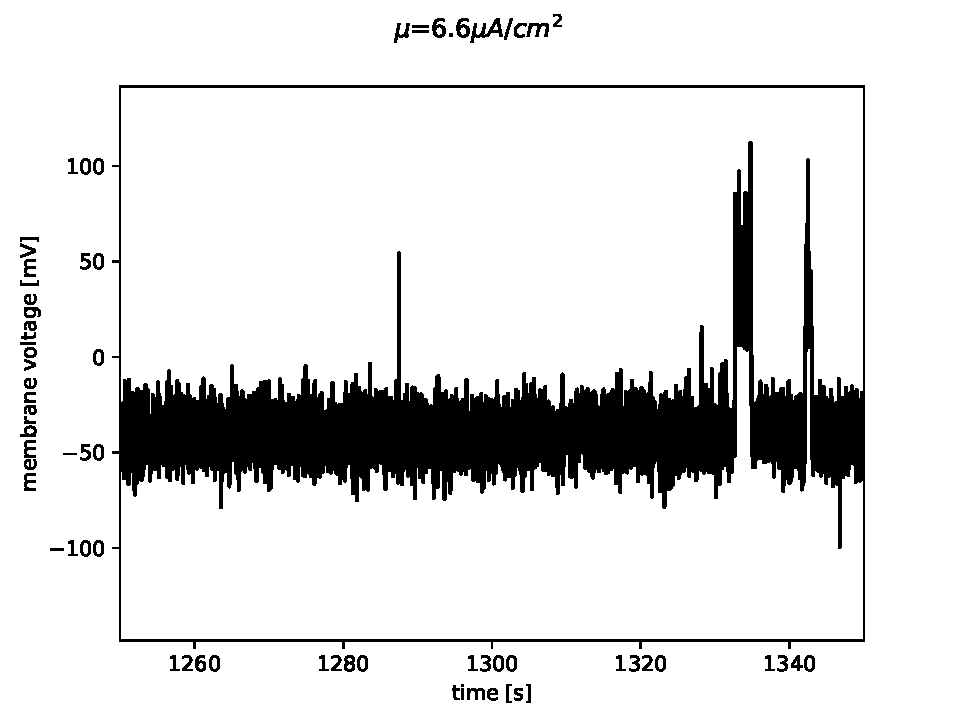
\includegraphics[scale=1]{realstaterinzel.pdf}\caption{Spannungsvariable im vereinfachten H-H}
	\label{rinzelvolt}
\end{figure}
\begin{figure}[H]
	\centering
	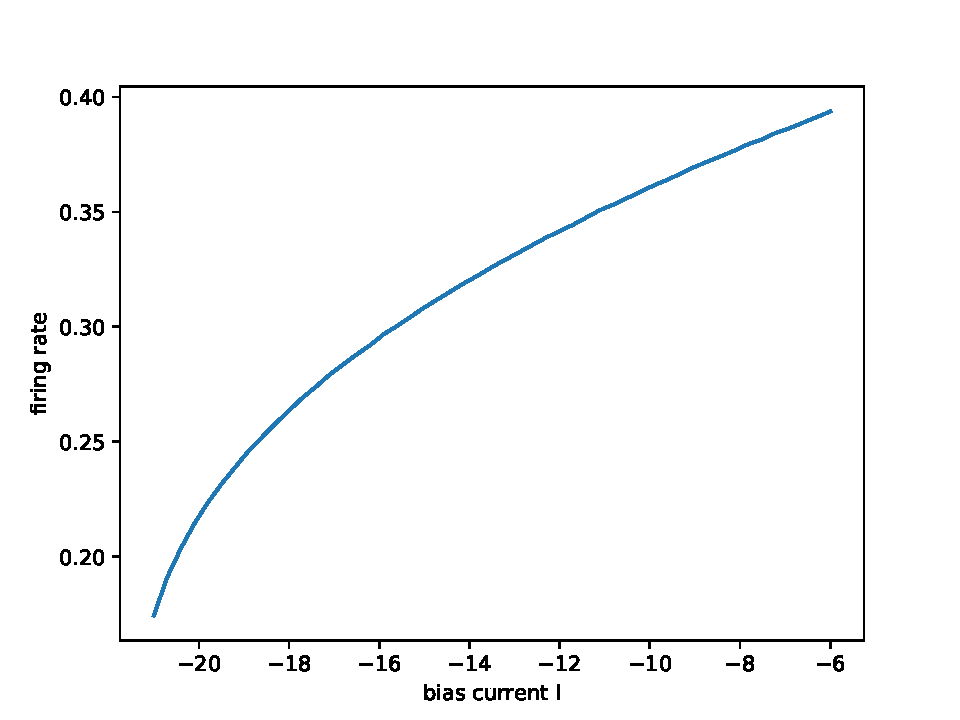
\includegraphics[scale=1]{detmocountrinzel.pdf}\caption{Verhalten der mittleren Feuerrate im vereinfachten H-H}
	\label{rinzelcount}
\end{figure}
\subsection{Zählstatistik}
\begin{figure}[H]
	\centering
	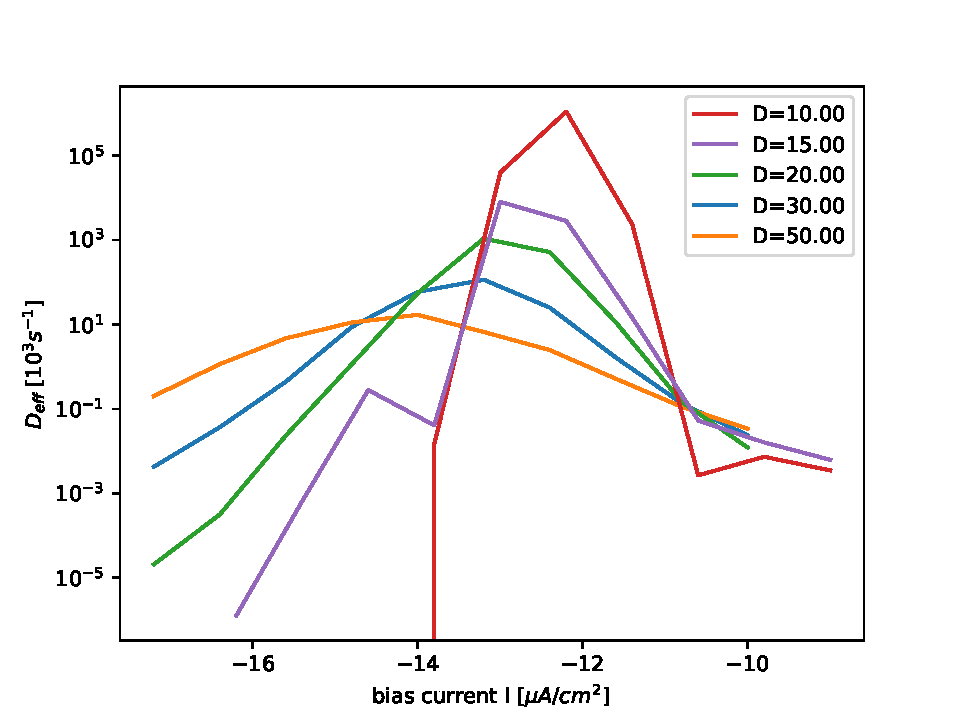
\includegraphics[scale=1]{drinzel.pdf}\caption{Verhalten des Diffusionskoeffizienten im vereinfachten H-H}
	\label{drinzel}
\end{figure}
\begin{figure}[H]
	\centering
	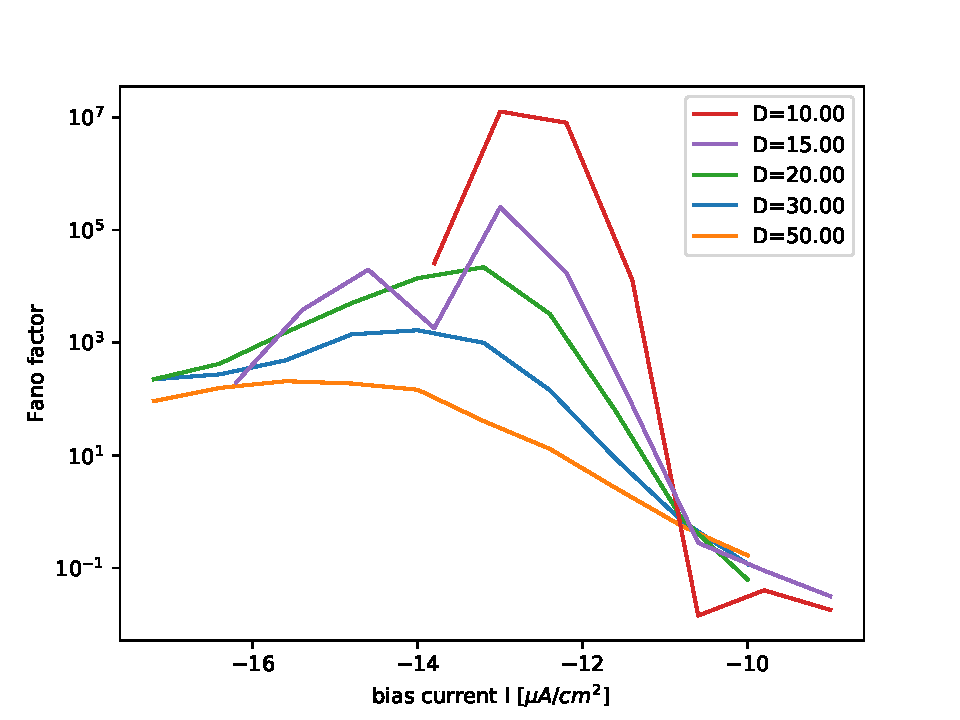
\includegraphics[scale=1]{frinzel.pdf}\caption{Verhalten des Fano-Faktors im vereinfachten H-H}
	\label{frinzel}
\end{figure}
\begin{figure}[H]
	\centering
	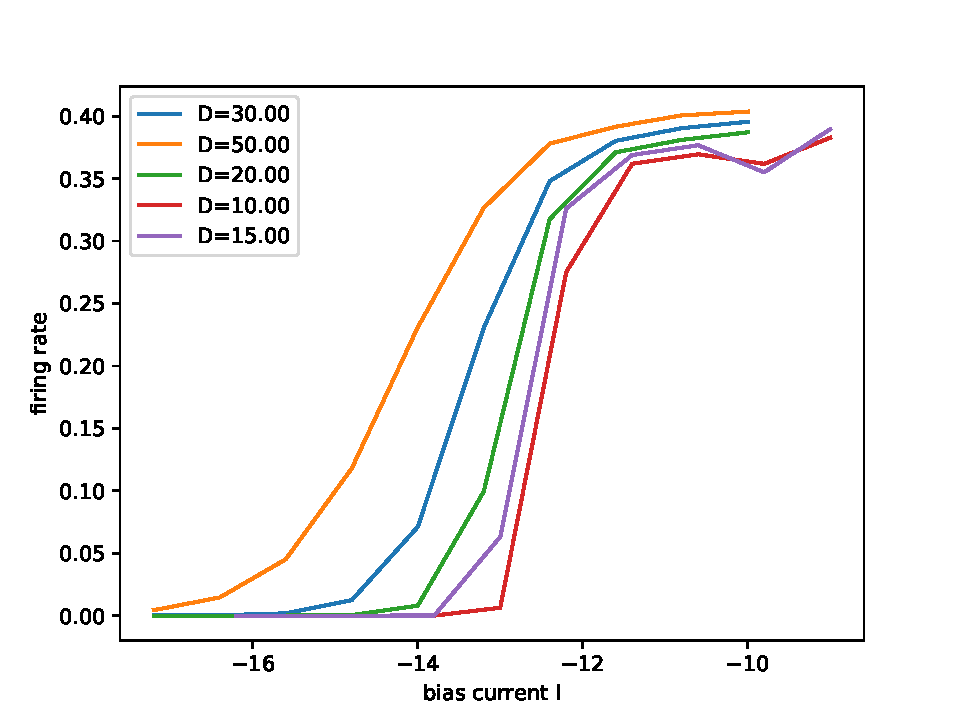
\includegraphics[scale=1]{grinzel.pdf}\caption{Verhalten der Feuerrate im vereinfachten H-H}
	\label{grinzel}
\end{figure}
\subsection{Zwei-Zustands-Theorie}
\begin{figure}[H]
	\centering
	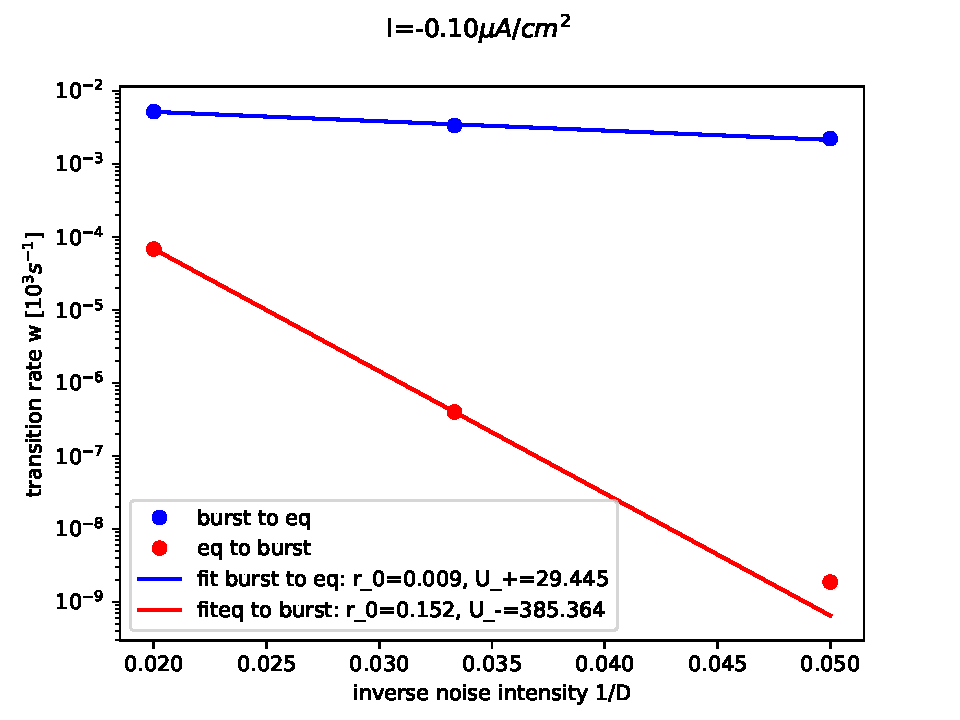
\includegraphics[scale=1]{arrheniustotrealrinzel25onewrealfast19jjem2stfit0.pdf}\caption{Übergangsraten bei kleinem Strom im vereinfachten H-H}
	\label{arrhrinzel1}
\end{figure}
\begin{figure}[H]
	\centering
	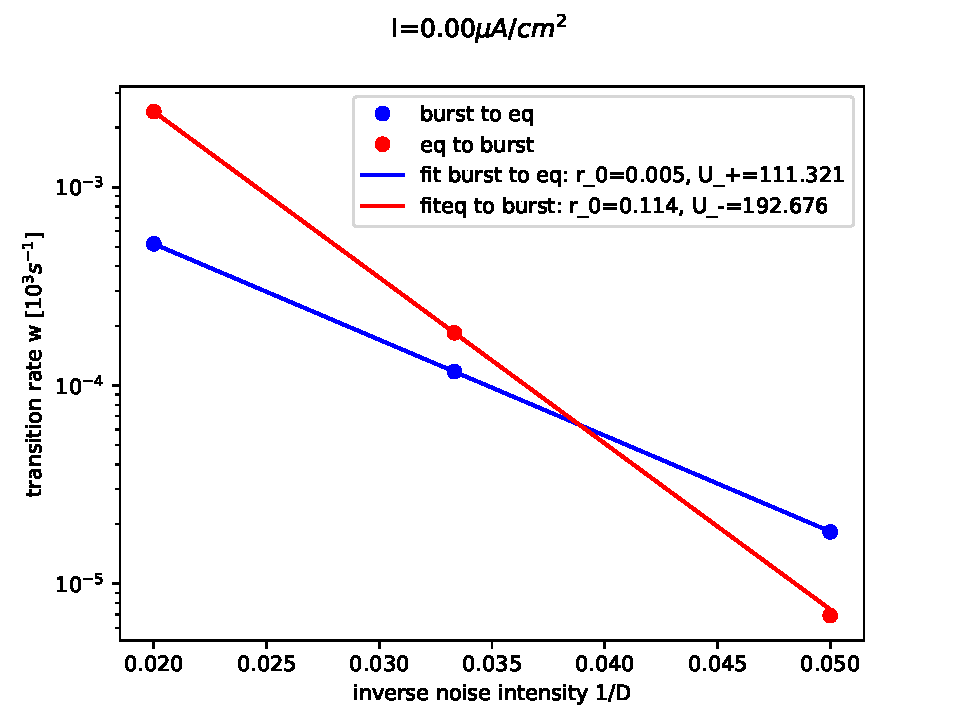
\includegraphics[scale=1]{arrheniustotrealrinzel25onewrealfast19jjem2stfit5.pdf}\caption{Übergangsraten bei mittlerem Strom im vereinfachten H-H}
	\label{arrhrinzel2}
\end{figure}
\begin{figure}[H]
	\centering
	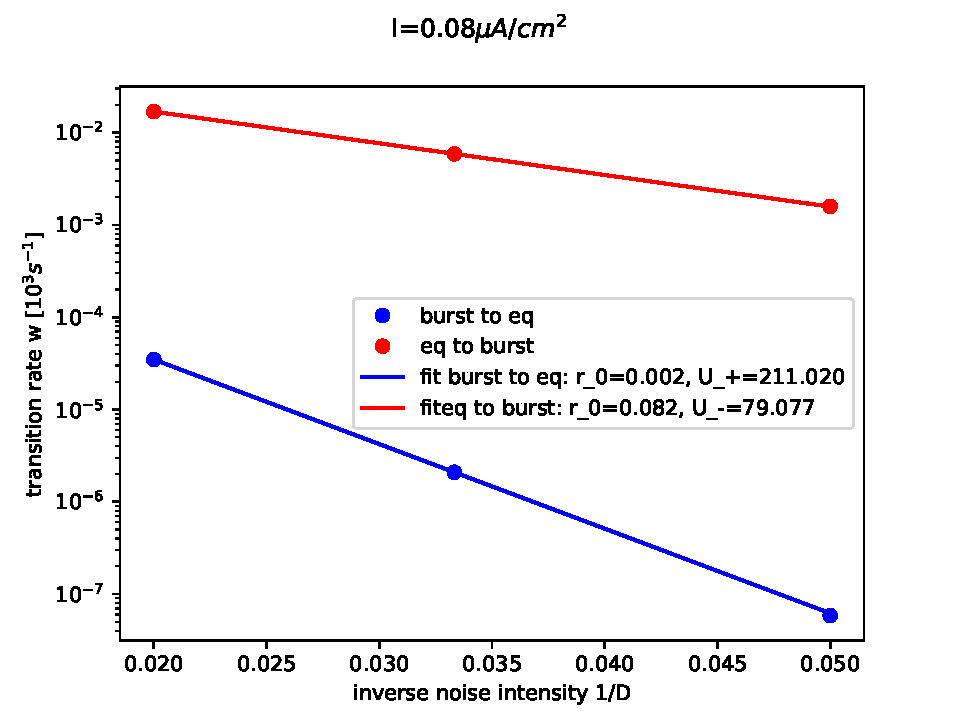
\includegraphics[scale=1]{arrheniustotrealrinzel25onewrealfast19jjem2stfit9.pdf}\caption{Übergangsraten bei hohem Strom im vereinfachten H-H}
	\label{arrhrinzel3}
\end{figure}
\begin{figure}[H]
	\centering
	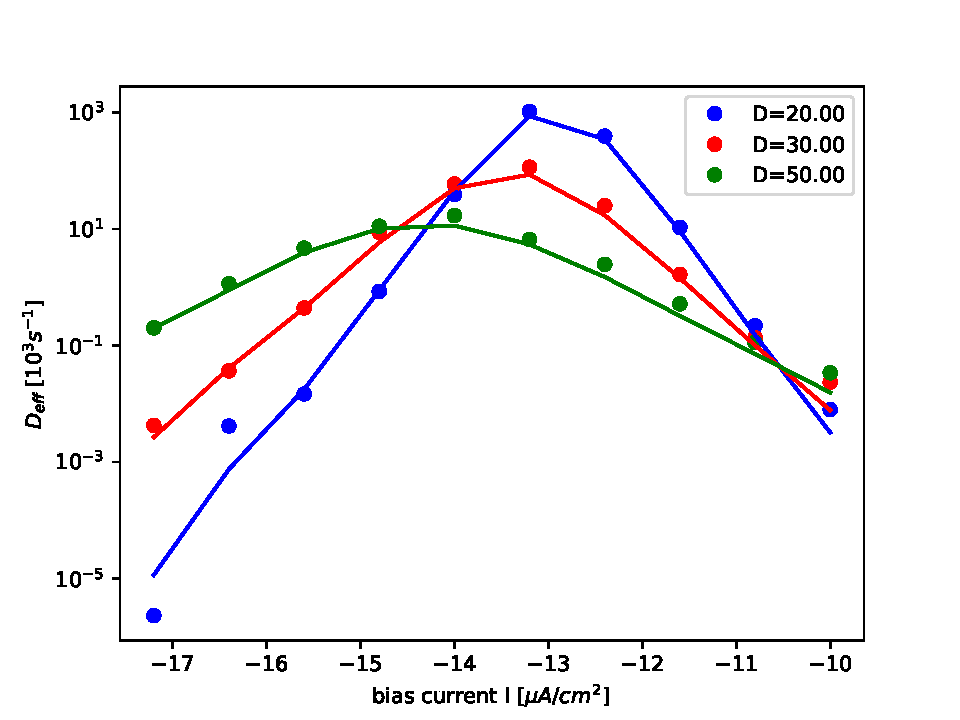
\includegraphics[scale=1]{dcompdfpwnewrealrinzel25orealfast19jjem2st.pdf}\caption{Vergleich des Diffusionskoeffizienten mit Zwei-Zustands-Modell im vereinfachten H-H}
	\label{drinzelcomp}
\end{figure}
\begin{figure}[H]
	\centering
	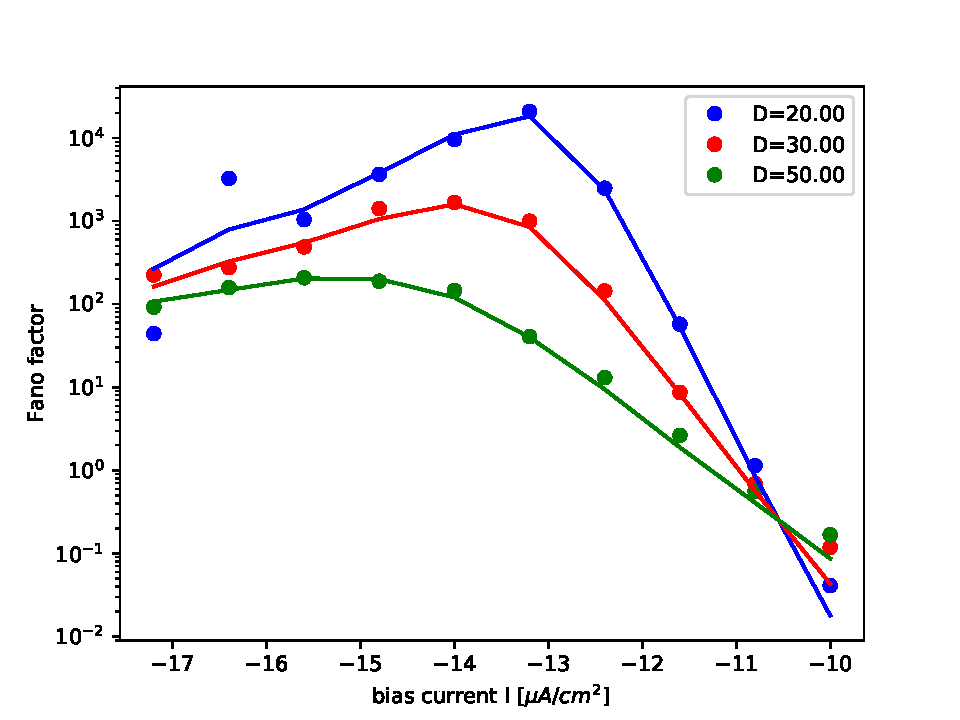
\includegraphics[scale=1]{fcompdfpwnewrealrinzel25orealfast19jjem2st.pdf}\caption{Vergleich des Fano-Faktors mit Zwei-Zustands-Modell im vereinfachten H-H}
	\label{frinzelcomp}
\end{figure}
\begin{figure}[H]
	\centering
	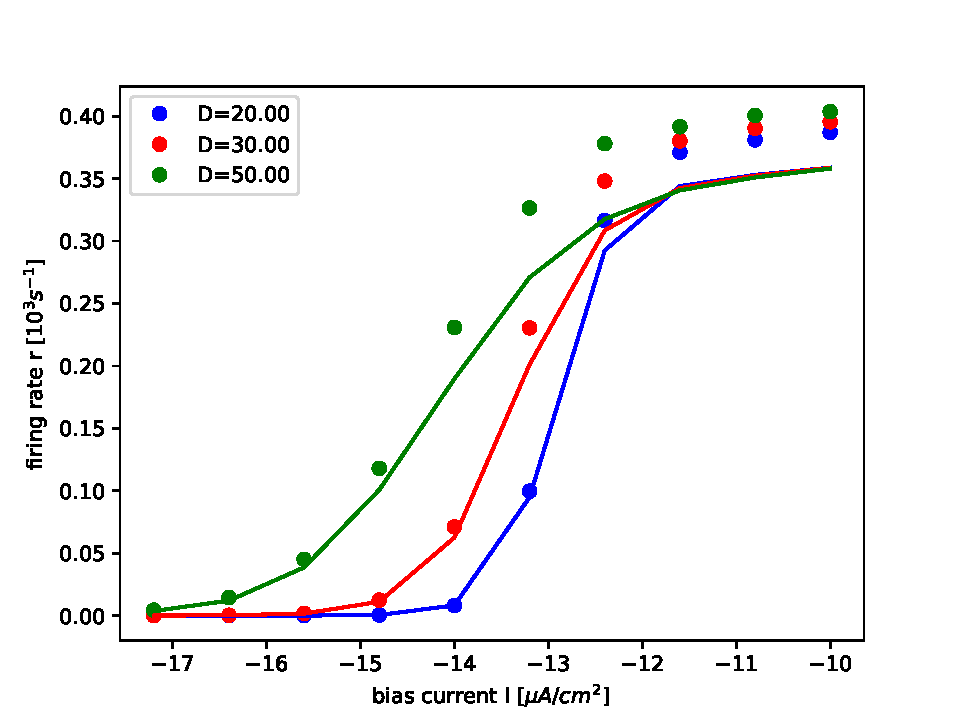
\includegraphics[scale=1]{gcompdfpwnewrealrinzel25orealfast19jjem2st.pdf}\caption{Vergleich der Feuerrate mit Zwei-Zustands-Modell im vereinfachten H-H}
	\label{grinzelcomp}
\end{figure}
\subsection{Wahl der Anfangsbedingungen}
\begin{figure}[H]
	\centering
	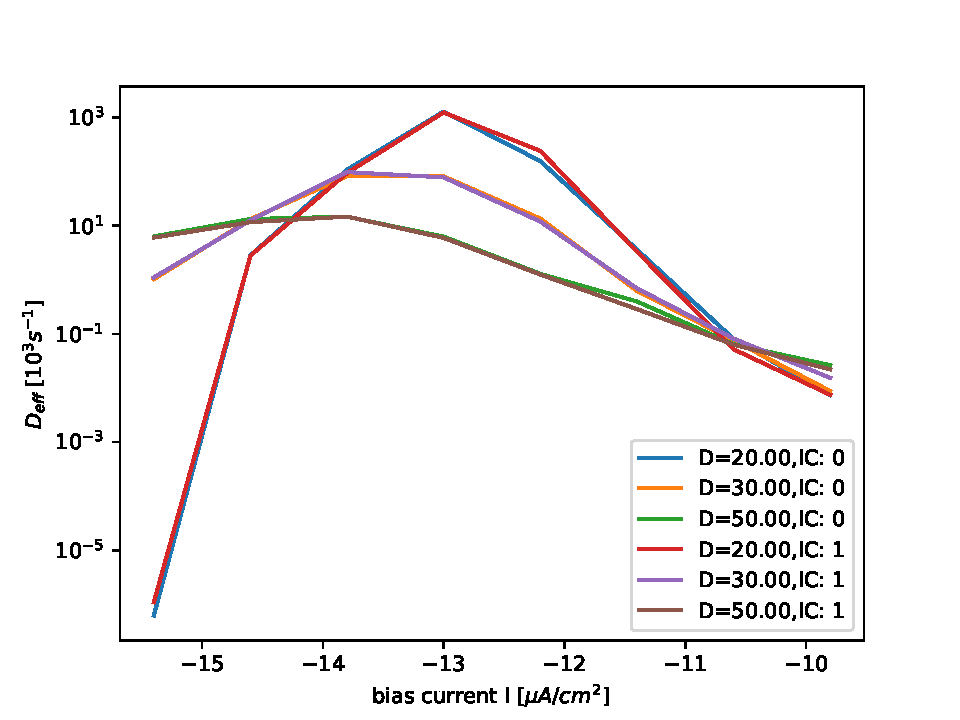
\includegraphics[scale=1]{dneursinglerealrinzel15ninv0realrinzel15ninv1.pdf}\caption{Diffusionskoeffizient bei verschiedenen AB}
	\label{drinzelab}
\end{figure}
\begin{figure}[H]
	\centering
	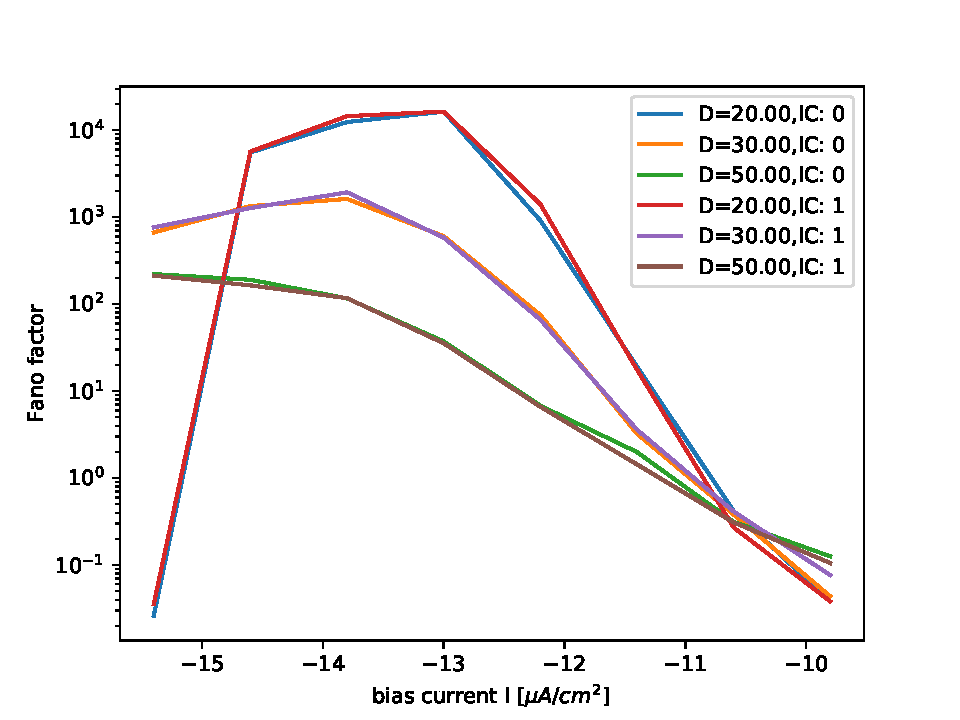
\includegraphics[scale=1]{fneursinglerealrinzel15ninv0realrinzel15ninv1.pdf}\caption{Fano-Faktor bei verschiedenen AB}
	\label{frinzelab}
\end{figure}
\begin{figure}[H]
\centering
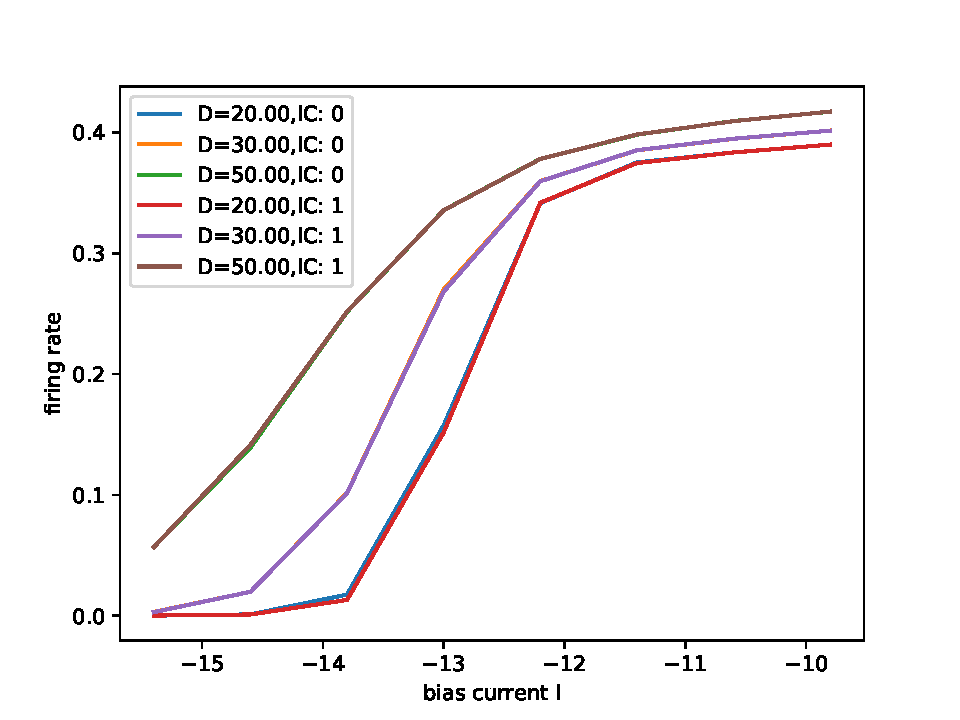
\includegraphics[scale=1]{gneursinglerealrinzel15ninv0realrinzel15ninv1.pdf}\caption{Feuerrate bei verschiedenen AB}
\label{grinzelab}
\end{figure}
\begin{figure}[H]
	\centering
	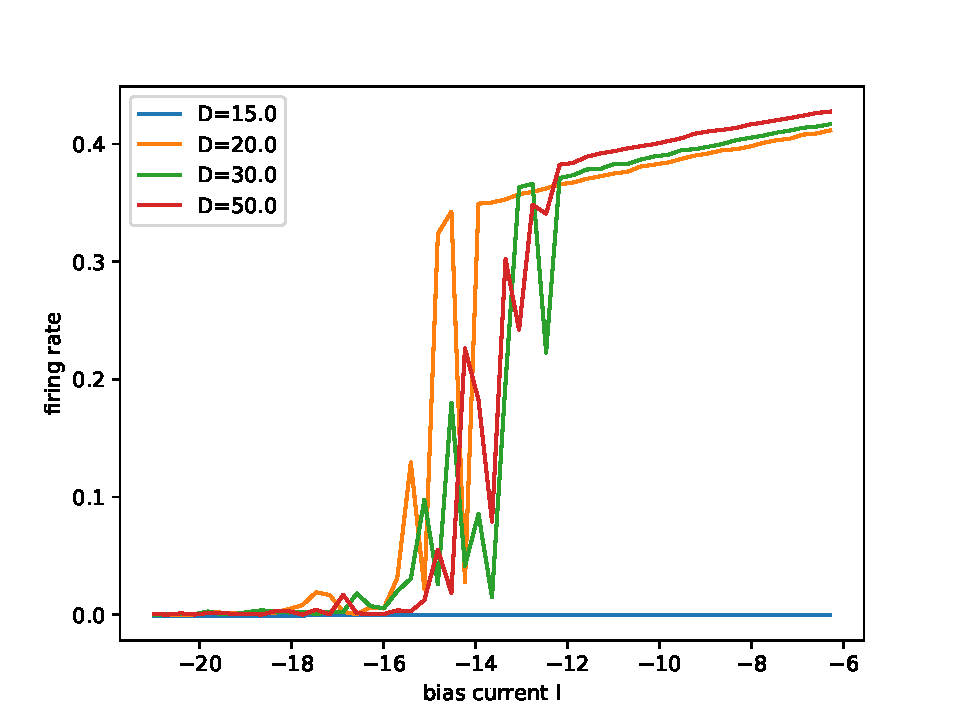
\includegraphics[scale=1]{firingraterinzelnoise3.pdf}\caption{Feuerrate im laufenden Zustand bei verschiedenen Rauschintensitäten}
	\label{gnoise}
\end{figure}
\subsection{SNR}
\subsubsection{Absch"atzung aus $D_{eff}$ und r}
\begin{figure}[H]
	\centering
	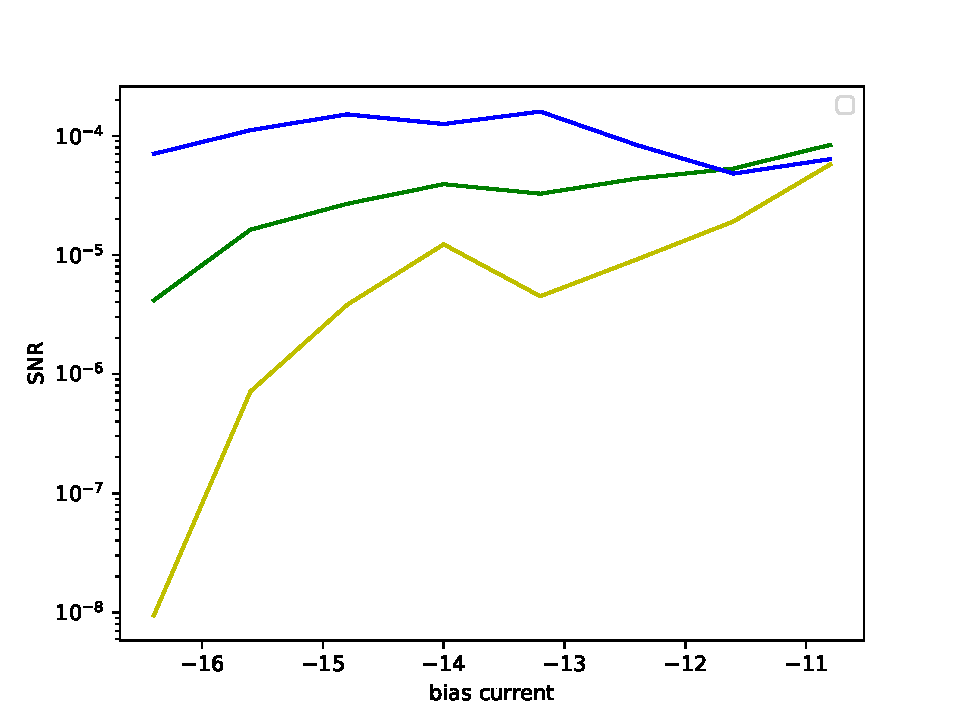
\includegraphics[scale=1]{snrangerealrinzel.pdf}\caption{Abschätzung des SNR aus $D_{eff}$ und der num. Ableitung von r}
	\label{rinzelabsch}
\end{figure}
\begin{figure}[H]
	\centering
	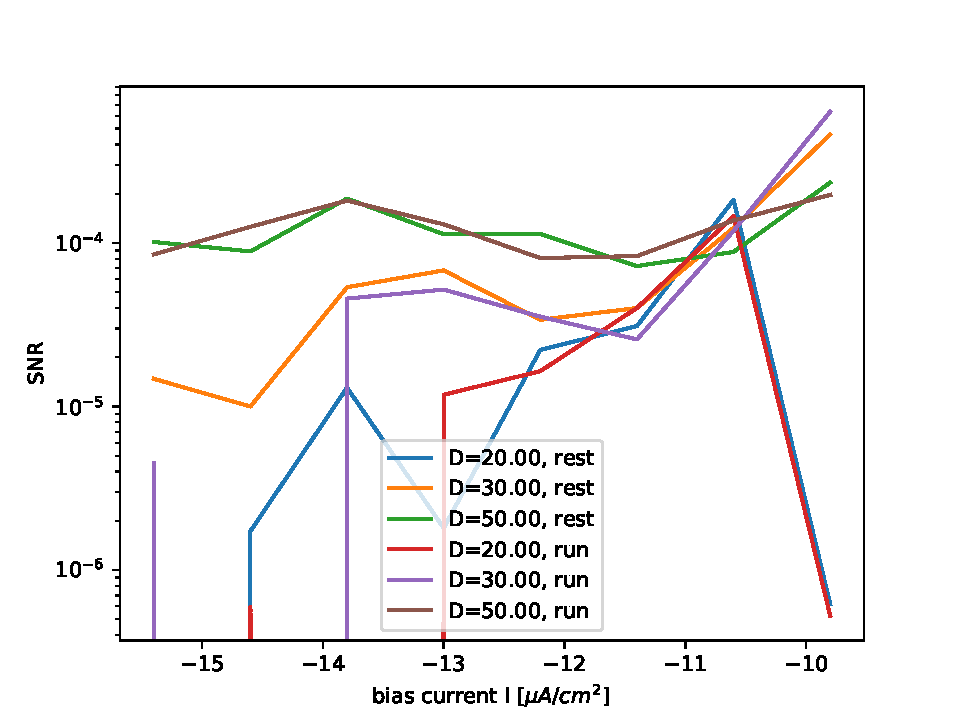
\includegraphics[scale=1]{snronlyrinzel.pdf}\caption{Messung des SNR aus dem Leistungsspektrum}
	\label{rinzelmeas}
\end{figure}
\begin{figure}[H]
	\centering
	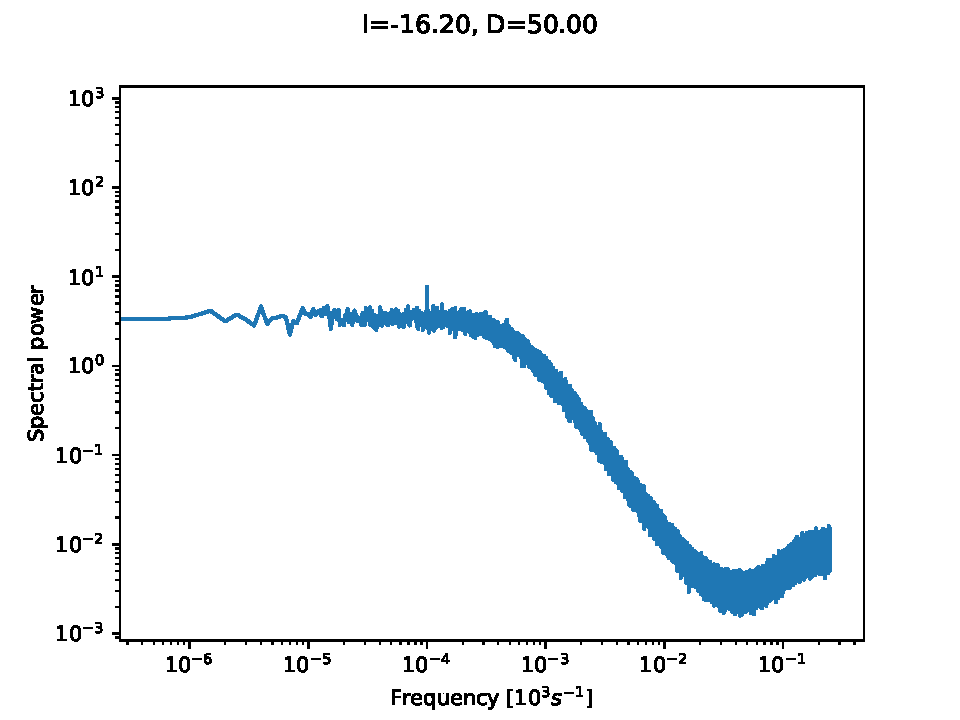
\includegraphics[scale=1]{fourd5small.pdf}\caption{Leistungsspektrum bei kleinem Strom}
	\label{fourd5s}
\end{figure}
\begin{figure}[H]
\centering
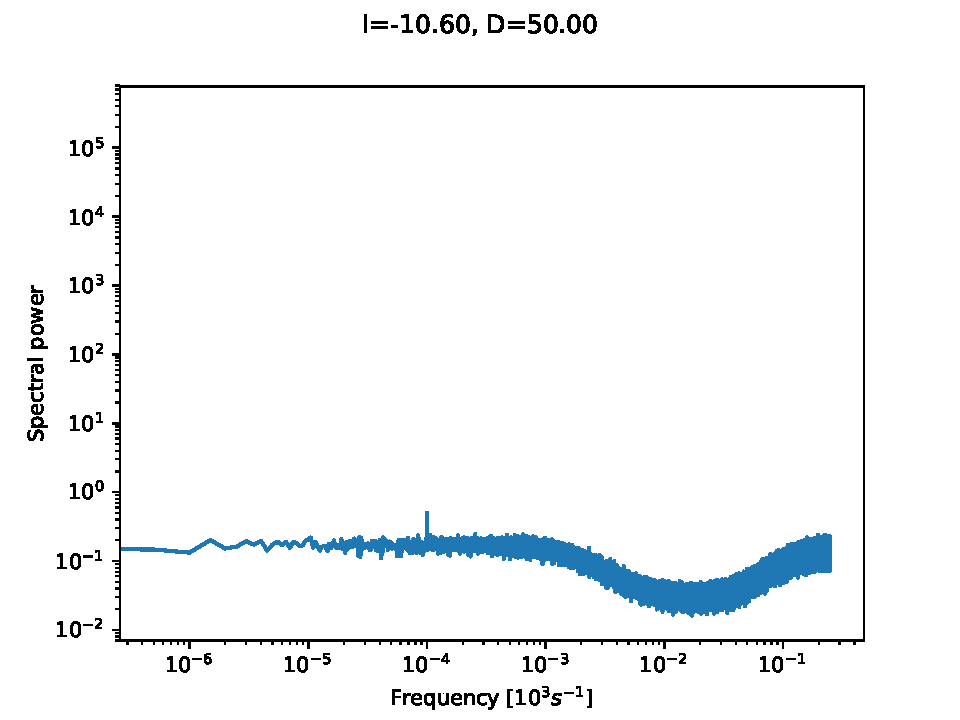
\includegraphics[scale=1]{fourd5large.pdf}\caption{Leistungsspektrum bei hohem Strom}
\label{fourd5h}
\end{figure}
\begin{figure}[H]
\centering
\includegraphics[scale=1]{fourd3small.pdf}\caption{Leistungsspektrum bei kleinem Strom}
\label{fourd3s}
\end{figure}
\begin{figure}[H]
	\centering
	\includegraphics[scale=1]{fourd3large.pdf}\caption{Leistungsspektrum bei hohem Strom}
	\label{fourd3h}
\end{figure}
\begin{figure}[H]
	\centering
	\includegraphics[scale=1]{snrangerealrinzel.pdf}\caption{Abschätzung des SNR aus $D_{eff}$ und der num. Ableitung von r}
	\label{rinzelabsch2}
\end{figure}
\begin{figure}[H]
	\centering
	\includegraphics[scale=1]{snronlyrinzelrealrinzel20ninv0.pdf}\caption{Abschätzung des SNR aus $D_{eff}$ und der num. Ableitung von r}
	\label{snr20n}
\end{figure}
\begin{figure}[H]
	\centering
	\includegraphics[scale=1]{d20i98.pdf}\caption{SNR bei hohem Strom}
	\label{spek209}
\end{figure}
\begin{figure}[H]
	\centering
	\includegraphics[scale=1]{d20i106.pdf}\caption{SNR bei hohem Strom}
	\label{spek208}
\end{figure}
\begin{figure}[H]
	\centering
	\includegraphics[scale=1]{d20i146.pdf}\caption{SNR bei hohem Strom}
	\label{spek203}
\end{figure}
\begin{figure}[H]
	\centering
	\includegraphics[scale=1]{d20i154.pdf}\caption{SNR bei hohem Strom}
	\label{spek202}
\end{figure}
\newpage
\begin{figure}[H]
	\centering
	\includegraphics[scale=1]{detmocountrinzelcomp2.pdf}\caption{Rauschabhängige Feuerraten im laufenden Zustand}
	\label{detrinzelrate}
\end{figure}
\begin{figure}[H]
	\centering
	\includegraphics[scale=1]{gcomprate3nolog.pdf}\caption{Mittlere rauschabhängige Feuerraten mit Vorhersage}
	\label{rinzelrate}
\end{figure}
\begin{figure}[H]
	\centering
	\includegraphics[scale=1]{raterinzelfit3.pdf}\caption{Fit der Vorfaktoren der Raten}
	\label{ratefit}
\end{figure}
\begin{figure}[H]
	\centering
	\includegraphics[scale=1]{barrierinzelfit3.pdf}\caption{Fit der Potenzialbarrieren}
	\label{barrierfit}
\end{figure}
\begin{figure}[H]
	\centering
	\includegraphics[scale=1]{snrangerealrinzelcomp.pdf}\caption{Vergleich SNR mit Abschätzung aus $D_{eff}$ und numerischer Ableitung der Raten}
	\label{snrinzelcomp}
\end{figure}
\begin{figure}[H]
	\centering
	\includegraphics[scale=1]{drdirinzel.pdf}\caption{Numerische Ableitung der Raten}
	\label{drdirin}
\end{figure}

\begin{figure}[H]
	\centering
	\includegraphics[scale=1]{dcompdfpwnewrealrinzel25orealrinzel15ninv0.pdf}\caption{Diffusionskoeffizient mit Punkt-für-Punkt-Vorhersage}
	\label{drin}
\end{figure}
\begin{figure}[H]
	\centering
	\includegraphics[scale=1]{dcomprate25o.pdf}\caption{Diffusionskoeffizient mit analytischer Vorhersage (ohne Signal)}
	\label{drinana}
\end{figure}
\begin{figure}[H]
	\centering
	\includegraphics[scale=1]{snrinzelcompsprate4.pdf}\caption{Vergleich SNR mit Abschätzung der Zwei-Zustands-Theorie}
	\label{snrinzelcomprate}
\end{figure}
\begin{figure}[H]
	\centering
	\includegraphics[scale=1]{inapikpoi.pdf}\caption{Leistungsspektrum nahe des Schnittpunktes}
	\label{inapikpoi}
\end{figure}
\begin{figure}[H]
	\centering
	\includegraphics[scale=1]{snrinzelcompspratepoi2.pdf}\caption{Vergleich SNR mit Abschätzung der Zwei-Zustands-Theorie}
	\label{snrinzelcompratepoi}
\end{figure}
\begin{figure}[H]
	\centering
	\includegraphics[scale=1]{arrheniustotrealrinzelpoi26n1realrinzel15ninv0fit4.pdf}\caption{Arrheniusfit nahe des Schnittpunktes}
	\label{arrhpoi}
\end{figure}
\begin{figure}[H]
	\centering
	\includegraphics[scale=1]{dcomprate3.pdf}\caption{Diffusionskoeffizient mit analytischer Vorhersage (mit Signal)}
	\label{drinanasig}
\end{figure}
\begin{figure}[H]
	\centering
	\includegraphics[scale=1]{bdistajrj2realrinzelpoi26n13001.pdf}\caption{Verteilung der burstenden Intervalle bei $D=30$}
	\label{b3001}
\end{figure}
\begin{figure}[H]
	\centering
	\includegraphics[scale=1]{bdistajrj2realrinzelpoi26n14003.pdf}\caption{Verteilung der burstenden Intervalle bei $D=40$}
	\label{b4003}
\end{figure}
\begin{figure}[H]
	\centering
	\includegraphics[scale=1]{eqdistajrj2realrinzelpoi26n11501.pdf}\caption{Verteilung der ruhenden Intervalle bei $D=15$}
	\label{eq1501}
\end{figure}
\begin{figure}[H]
	\centering
	\includegraphics[scale=1]{eqdistajrj2realrinzelpoi26n12001.pdf}\caption{Verteilung der burstenden Intervalle bei $D=20$}
	\label{eq2001}
\end{figure}
\newpage
\begin{figure}[H]
	\centering
	\includegraphics[scale=1]{firingraterinzelnoiselong.pdf}\caption{Numerische Bestimmung der Feuerraten}
	\label{firatenoise}
\end{figure}
\begin{figure}[H]
	\centering
	\includegraphics[scale=1]{firingraterinzelnoiselonglog.pdf}\caption{Numerische Bestimmung der Feuerraten in logarithmischer Darstellung}
	\label{firatenoiselog}
\end{figure}
\begin{figure}[H]
\centering
\includegraphics[scale=1]{drdirinzel.pdf}\caption{Numerische Ableitung der Raten mit grober Auflösung}
\label{drdirin2}
\end{figure}
\begin{figure}[H]
	\centering
	\includegraphics[scale=1]{drdirinzellong.pdf}\caption{Numerische Bestimmung des Betrags der Ableitung}
	\label{firatenoisederiv}
\end{figure}
\begin{figure}[H]
	\centering
	\includegraphics[scale=1]{snrangerealrinzelcomp.pdf}\caption{Vergleich SNR mit Abschätzung aus $D_{eff}$ und numerischer Ableitung der Raten}
	\label{snrinzelcomp2}
\end{figure}
\begin{figure}[H]
	\centering
	\includegraphics[scale=1]{snrangerealrinzelcomplong.pdf}\caption{Vergleich SNR mit Abschätzung aus $D_{eff}$ und numerischer Ableitung der Raten mit höherer Auflösung}
	\label{snrinzelcomplong}
\end{figure}
\begin{figure}[H]
	\centering
	\includegraphics[scale=1]{spekpoi4dd20.pdf}\caption{Leistungsspektrum mit geringerer Signalamplitude ($\epsilon=0.3$)}
	\label{spekpoi20}
\end{figure}
\begin{figure}[H]
	\centering
	\includegraphics[scale=1]{spekpoi4dd30.pdf}\caption{Leistungsspektrum mit geringerer Signalamplitude ($\epsilon=0.3$)}
	\label{spekpoi30}
\end{figure}
\begin{figure}[H]
	\centering
	\includegraphics[scale=1]{snrinzelpoi4d3.pdf}\caption{Vergleich SNR mit Zwei-Zustands-Theorie}
	\label{snrpoi4d}
\end{figure}
\begin{figure}[H]
	\centering
	\includegraphics[scale=1]{arrhcomp.pdf}\caption{Vergleich der Übergangsraten mit und ohne Signal}
	\label{arrhratecomp}
\end{figure}
\newpage
\subsection{SNR am Schnittpunkt}
schwächeres Signal, längere Simulationszeit
\begin{figure}[H]
	\centering
	\includegraphics[scale=1]{inapikrealrD20I-114.pdf}\caption{Spektrum für Strom unter dem Schnittpunkt}
	\label{rinzelsnrpois}
\end{figure}
\begin{figure}[H]
	\centering
	\includegraphics[scale=1]{inapikrealrD30I-102.pdf}\caption{Spektrum für Strom über dem Schnittpunkt}
	\label{rinzelsnrpoil}
\end{figure}
\begin{figure}[H]
	\centering
	\includegraphics[scale=1]{snrinzelpoi6j17d.pdf}\caption{SNR nahe Schnittpunkt für alle untersuchten Rauschintensitäten}
	\label{rinzelsnrpoitot}
\end{figure}
\begin{figure}[H]
	\centering
	\includegraphics[scale=1]{snrinzelpoi6j17dshort.pdf}\caption{SNR nahe Schnittpunkt für Auswahl verschiedener D}
	\label{rinzelsnrpoisel}
\end{figure}
\subsubsection{Vergleich $D_{eff}$ Zwei-Zustands-Theorie}
\begin{figure}[H]
	\centering
	\includegraphics[scale=1]{dcomprate25o6j.pdf}\caption{Vergleich Diffusionskoeffizient mit Zwei-Zustands-Theorie}
	\label{dcompraterinzel}
\end{figure}
\begin{figure}[H]
	\centering
	\includegraphics[scale=1]{gcomprate25o6jnolog.pdf}\caption{Vergleich mittlere Feuerrate mit Zwei-Zustands-Theorie}
	\label{gcompraterinzel}
\end{figure}
\begin{figure}[H]
	\centering
	\includegraphics[scale=1]{gcompratepoi17dnolog.pdf}\caption{Vergleich mittlere Feuerrate unter Signal mit Zwei-Zustands-Theorie}
	\label{gcompraterinzelsig}
\end{figure}
\begin{figure}[H]
	\centering
	\includegraphics[scale=1]{barrierinzelfit4.pdf}\caption{Neuer Fit der Potentialbarrieren}
	\label{barrierinzelfit}
\end{figure}
\newpage
\subsubsection{Übergangsraten in Abhängigkeit vom Strom}
\begin{figure}[H]
	\centering
	\includegraphics[scale=1]{tranrates.pdf}\caption{Übergangsraten für das Modell nach Rinzel}
	\label{tranraterinzel}
\end{figure}
\begin{figure}[H]
	\centering
	\includegraphics[scale=1]{tranratesneur.pdf}\caption{Übergangsraten für das $I_{Na,p}+I_K$ Modell}
	\label{tranrateneur}
\end{figure}
\subsubsection{Verifikation: Spektrum eines OUP}
\begin{figure}[H]
	\centering
	\includegraphics[scale=1]{oup2jtheo3.pdf}\caption{Leistungsspektrum eines OUP mit Theorie}
	\label{oupsp}
\end{figure}
\subsubsection{Phasenraum}
\begin{figure}[H]
	\centering
	\includegraphics[scale=1]{rinzelclines.pdf}\caption{Numerisch bestimmte Isoklinen des Rinzel-Modells bei $I_{app}=-12$}
	\label{rinzelclines}
\end{figure}
\begin{figure}[H]
	\centering
	\includegraphics[scale=1]{rinzelclinescor.pdf}\caption{Numerisch bestimmte Isoklinen bei $I_{app}=-12$ mit Ausschlusskriterium $W(V)<0.01$}
	\label{rinzelclinescor}
\end{figure}
\begin{figure}[H]
	\centering
	\includegraphics[scale=1]{rinzelclinescoredge2.pdf}\caption{Numerisch bestimmte Isoklinen bei $I_{app}=-6$ mit Ausschlusskriterium $W(V)<0.01$}
	\label{rinzelclinescoredge}
\end{figure}
\begin{figure}[H]
	\centering
	\includegraphics[scale=1]{snrinzelrange26d.pdf}\caption{Vergleich SNR mit Zwei-Zustands-Theorie über nahezu gesamten Bereich der Bistabilität}
	\label{snrange}
\end{figure}
\subsection{Subkritische Andronov-Hopf Bifurkation}
\begin{figure}[H]
	\centering
	\includegraphics[scale=1]{dneurrealanhopf22j3.pdf}\caption{Effektiver Diffusionskoeffizient im $I_{Na,p}+I_K$ - Modell mit subkritischer AH-Bifurkation}
	\label{deffanhopf}
\end{figure}
\begin{figure}[H]
	\centering
	\includegraphics[scale=1]{gneurrealanhopf22j3.pdf}\caption{Mittlere Feuerrate im $I_{Na,p}+I_K$ - Modell mit subkritischer AH-Bifurkation}
	\label{ganhopf}
\end{figure}
\begin{figure}[H]
	\centering
	\includegraphics[scale=1]{fneurrealanhopf22j3.pdf}\caption{Fano-Faktor im $I_{Na,p}+I_K$ - Modell mit subkritischer AH-Bifurkation}
	\label{fanoanhopf}
\end{figure}
\subsection{SNR im subkritschen AH-Modell}
\begin{figure}[H]
	\centering
	\includegraphics[scale=1]{spanhopfd10klein.pdf}\caption{Leistungsspektrum bei geringem Strom}
	\label{powerspD01klein}
\end{figure}
\begin{figure}[H]
	\centering
	\includegraphics[scale=1]{spanhopfd10mittel.pdf}\caption{Leistungsspektrum bei mittlerem Strom}
	\label{powerspD01mittel}
\end{figure}
\begin{figure}[H]
	\centering
	\includegraphics[scale=1]{spanhopfd10mittel2.pdf}\caption{Leistungsspektrum bei mittlerem Strom}
	\label{powerspD01mittel2}
\end{figure}
\begin{figure}[H]
	\centering
	\includegraphics[scale=1]{spanhopfd10hoch.pdf}\caption{Leistungsspektrum bei hohem Strom}
	\label{powerspD01hoch}
\end{figure}
\begin{figure}[H]
	\centering
	\includegraphics[scale=1]{spanhopfd20klein.pdf}\caption{Leistungsspektrum bei geringem Strom}
	\label{powerspD02klein}
\end{figure}
\begin{figure}[H]
	\centering
	\includegraphics[scale=1]{spanhopfd30hoch.pdf}\caption{Leistungsspektrum bei hohem Strom}
	\label{powerspD03hoch}
\end{figure}
\begin{figure}[H]
	\centering
	\includegraphics[scale=1]{snranhopf27jws.pdf}\caption{SNR für zwei verschiedene Rauschintensitäten}
	\label{snranhopf}
\end{figure}
Problem: Fouriertrafo wird nicht mit allen Punkten durchgeführt, sondern nur mit einer äquidistanten Auswahl von Punkten. Überschreitet das Zeitintervall dieses Samplings die Periodenlänge des Feuerns, kann die Feuerrate nicht mehr aus dem Spektrum abgelesen werden.
\\
Lösung: Erhöhen der Sampling-Rate:
\begin{figure}[H]
	\centering
	\includegraphics[scale=1]{spanhopfd20ismallwlim.pdf}\caption{Leistungsspektrum des $I_{Na,p}+I_K$ - Modells mit Andronov-Hopf Bifurkation bei geringem Bias-Strom}
	\label{spanhopfismall}
\end{figure}
\begin{figure}[H]
	\centering
	\includegraphics[scale=1]{spanhopfd20imediumwlim.pdf}\caption{Leistungsspektrum des $I_{Na,p}+I_K$ - Modells mit Andronov-Hopf Bifurkation bei mittlerem Bias-Strom}
	\label{spanhopfimedium}
\end{figure}
\begin{figure}[H]
	\centering
	\includegraphics[scale=1]{spanhopfd30ilargewlim.pdf}\caption{Leistungsspektrum des $I_{Na,p}+I_K$ - Modells mit Andronov-Hopf Bifurkation bei hohem Bias-Strom}
	\label{spanhopfilarge}
\end{figure}
\section{Log-Spektrum}
\begin{figure}[H]
	\centering
	\includegraphics[scale=1]{logspecmed.pdf}\caption{Spektrum bei mittlerem Bias-Strom}
	\label{specmedlog}
\end{figure}
\begin{figure}[H]
	\centering
	\includegraphics[scale=1]{logspeclarge.pdf}\caption{Spektrum bei hohem Bias-Strom}
	\label{speclargelog}
\end{figure}
\begin{figure}[H]
	\centering
	\includegraphics[scale=1]{dneurrealanhopf22j3.pdf}\caption{Effektiver Diffusionskoeffizient im $I_{Na,p}+I_K$ - Modell mit subkritischer AH-Bifurkation}
	\label{deffanhopf2}
\end{figure}
\begin{figure}[H]
	\centering
	\includegraphics[scale=1]{snrangerealanameasspallanhopf.pdf}\caption{Vergleich numerisches SNR mit Abschätzung aus $D_{eff}$ und Feuerrate}
	\label{snranhopflog}
\end{figure}
\subsection{Kombination der Spektren}
\begin{figure}[H]
	\centering
	\includegraphics[scale=1]{twofoud35i4375os.pdf}\caption{Leistungsspektra bei geringem Strom im $I_{Na}+I_K$-Modell mit subkrit. Andronov-Hopf-Bifurkation}
	\label{twofoud35small}
\end{figure}
\begin{figure}[H]
	\centering
	\includegraphics[scale=1]{twofoud35i4575os.pdf}\caption{Leistungsspektra bei mittlerem Strom im $I_{Na}+I_K$-Modell mit subkrit. Andronov-Hopf-Bifurkation}
	\label{twofoud35medium}
\end{figure}
\begin{figure}[H]
	\centering
	\includegraphics[scale=1]{twofoud35i4775os.pdf}\caption{Leistungsspektra bei hohem Strom im $I_{Na}+I_K$-Modell mit subkrit. Andronov-Hopf-Bifurkation}
	\label{twofoud35large}
\end{figure}
\begin{figure}[H]
	\centering
	\includegraphics[scale=1]{twofoud20i4475ws.pdf}\caption{Leistungsspektra bei geringem Strom im $I_{Na}+I_K$-Modell mit subkrit. Andronov-Hopf-Bifurkation}
	\label{twofoud20small}
\end{figure}
\begin{figure}[H]
	\centering
	\includegraphics[scale=1]{twofoud20i4575ws.pdf}\caption{Leistungsspektra bei mittlerem Strom im $I_{Na}+I_K$-Modell mit subkrit. Andronov-Hopf-Bifurkation}
	\label{twofoud20medium}
\end{figure}
\begin{figure}[H]
	\centering
	\includegraphics[scale=1]{twofoud20i4725ws.pdf}\caption{Leistungsspektra bei hohem Strom im $I_{Na}+I_K$-Modell mit subkrit. Andronov-Hopf-Bifurkation}
	\label{twofoud20large}
\end{figure}
\begin{figure}[H]
	\centering
	\includegraphics[scale=1]{twofoud25i4450ws.pdf}\caption{Leistungsspektra bei geringem Strom im $I_{Na}+I_K$-Modell mit subkrit. Andronov-Hopf-Bifurkation}
	\label{twofoud25small}
\end{figure}
\subsection{$I_{Na,p}+I_K$ Modell mit Andronov-Hopf Bifurkation}
\subsubsection{Ecke bei $D=0.1$}
\begin{figure}[H]
	\centering
	\includegraphics[scale=1]{dneurrealanhopf21flogcornerrealanhopf19flog.pdf}\caption{Diffusionskoeffizient bei $D=0.1$}
	\label{deffanhopfcorner}
\end{figure}
\begin{figure}[H]
	\centering
	\includegraphics[scale=1]{fneurrealanhopf21flogcornerrealanhopf19flog.pdf}\caption{Fano-Faktor bei $D=0.1$}
	\label{fanoanhopfcorner}
\end{figure}
\subsubsection{Verbesserung der Frequenzauflösung im Spektrum}
\begin{figure}[H]
	\centering
	\includegraphics[scale=1]{freq200.pdf}\caption{Spektrum mit Auflösung von 200 Hz}
	\label{freq200}
\end{figure}
\begin{figure}[H]
	\centering
	\includegraphics[scale=1]{freq400.pdf}\caption{Spektrum mit Auflösung von 400 Hz}
	\label{freq400}
\end{figure}
\begin{figure}[H]
	\centering
	\includegraphics[scale=1]{freq800.pdf}\caption{Spektrum mit Auflösung von 800 Hz}
	\label{freq800}
\end{figure}
\begin{figure}[H]
	\centering
	\includegraphics[scale=1]{freq1600.pdf}\caption{Spektrum mit Auflösung von 1600 Hz}
	\label{freq1600}
\end{figure}
\begin{figure}[H]
	\centering
	\includegraphics[scale=1]{freq4000.pdf}\caption{Spektrum mit Auflösung von 4000 Hz}
	\label{freq4000}
\end{figure}
\subsubsection{SNR und Zwei-Zustands-Theorie}
\begin{figure}[H]
	\centering
	\includegraphics[scale=1]{snrtwostateanhopf3m.pdf}\caption{Vergleich SNR und 2-Zustands-Theorie}
	\label{snrtwostateanhopf}
\end{figure}
\end{document}